\documentclass[12pt]{article}

%To do list:
%%1) Fix numbering of reading problems from the reordering, e.g. Lecture 20, q1-->Lecture 18, q1
%%2) Rename webwork sets according to materials not lecture number
%%3) Move images into directories. Here
%%4) Webwork q5 HW6 (in MAT 67 ordering, say <,> for vector notation.
%%5) Problem 6, HW6 has a bug when the eigenvalue is 0.


%%%%%Some commands to make online notes...
\newcommand{\Lecture}{Module}
\newcommand{\moduletitle}[1]{\newpage\thispagestyle{empty}\begin{center}{\LARGE #1}\end{center}}
\newcommand{\modulesection}[1]{\thispagestyle{empty}\section{#1}}
\newcommand{\modulesubsection}[1]{\thispagestyle{empty}\subsection{#1}}
\newcommand{\modulecomment}[1]{}
\newcommand{\moduleobjectives}[1]{#1}
\newcommand{\inputProblems}[1]{}
\newcommand{\moduleinputProblems}[1]{\input{#1}}
\newcommand{\References}[1]{}
\newcommand{\moduletext}[2]{#2}

%use this if you need to show labels, but turn it off afterwards.
%\usepackage{showkeys}
%\usepackage{multimedia}
\usepackage{makeidx}
\usepackage{nopageno} 

\usepackage{comment}
\usepackage{shadow}
\usepackage[english]{babel}
\usepackage{blindtext}
\usepackage{graphicx, color}
\usepackage{tikz}
\DeclareGraphicsRule{*}{mps}{*}{}
\usepackage{linalgjh}
\usepackage{multirow}
\usepackage[colorlinks=true,linkcolor=blue,urlcolor=red,pdfnewwindow=true]{hyperref}
\usepackage[toc]{glossaries}
\usepackage{textcomp}
% Added to work with my enumerates, and I feel that it allows us more flexibility
%  to select how we want to number our items - TCS 1/9/12
\usepackage{enumerate}

\usepackage{linalgdir} % Get the directory and title information

%Change the next line as appropriate for your course.
\newcommand{\webworkurl}{http://webwork.math.ucdavis.edu/webwork2/MAT22A-Waldron-Winter-2012/}
%\newcommand{\webworkurl}{http://webwork.math.ucdavis.edu/webwork2/LinearAlgebra/}
\newcommand{\videourl}{http://math.ucdavis.edu/~linear/videos/}

% This command works by specifying the following (in order):
%  1 - the filename (with extension)
%  2 - the text describing the video
%  3 - The hyperlink reference
% For example we have
% \videoscriptlink{gaussian_elimination_more_background.mp4}{Augmented Matrix Notation~\ref{ge4} and~\ref{ge5}}{script_gaussian_elimination_more}
\newcommand{\videoscriptlink}[3]{
\begin{center}
\href{\videourl #1}{\raisebox{-.4cm}{
\includegraphics[scale=.075]{take1.jpg}}} \hspace{1cm}\scalebox{1.2}{\ttfamily #2}
\hspace{1cm} \hyperlink{#3}{\raisebox{-.3cm}{
\includegraphics[scale=.08]{script.jpg}}}
\end{center}
} % videoscriptlink definition
% I changed all videos I could find to this command - TCS 1/9/12

%%%This links to reading homeworks:
\newcommand{\reading}[2]{\begin{center}
\href{\webworkurl ReadingHomework#1/#2/}{
\raisebox{-3mm}{
\includegraphics[scale=.1]{glasses.jpg}}\hspace{2mm}Reading homework: problem #1.#2}\hspace{8mm}\end{center}}

%%%This links to Mark's videos
\newcommand{\markvideolink}[2]{
\begin{center}
\href{\videourl #1}{\raisebox{-.4cm}{
\includegraphics[scale=.075]{take1.jpg}}} \hspace{1cm}\scalebox{1.2}{\ttfamily #2}
\hspace{1cm} {\raisebox{-.3cm}{\includegraphics[scale=.2]{mark.jpg}}}
\end{center}
}


%%%This links to Kat's videos
\newcommand{\katvideolink}[2]{
\begin{center}
\href{\videourl #1}{\raisebox{-.4cm}{
\includegraphics[scale=.075]{take1.jpg}}} \hspace{1cm}\scalebox{1.2}{\ttfamily #2}
\hspace{1cm} {\raisebox{-.3cm}{\includegraphics[scale=.2]{kat.jpg}}}
\end{center}
}



%A simple URL macro
\newcommand{\URL}[1]{\begin{center}\href{#1}{\ttfamily\scriptsize #1}\end{center}}
\newcommand{\URLS}[2]{\begin{center}\href{#1}{\ttfamily\scriptsize #2}\end{center}}




\def\nn{\nonumber}

\newtheorem{theorem}{Theorem}[section]
\newtheorem{lemma}[theorem]{Lemma}
\newtheorem{proposition}[theorem]{Proposition}
\newtheorem{corollary}[theorem]{Corollary}


\newenvironment{definition}[1][Definition]{\begin{trivlist}
\item[\hskip \labelsep {\bfseries #1}]}{\end{trivlist}}
\newenvironment{example}[1][Example]{\small \sffamily \begin{trivlist}
\item[\hskip \labelsep {\bfseries #1}]}{\end{trivlist}}
\newenvironment{remark}[1][Remark]{\small \sffamily \begin{trivlist}
\item[\hskip \labelsep {\bfseries #1}]}{\end{trivlist}}

\DeclareMathOperator{\tr}{tr}
\DeclareMathOperator{\rref}{RREF}

% sideremark
\def\sideremark#1{\ifvmode\leavevmode\fi\vadjust{\vbox to0pt{\vss
\hbox to 0pt{\hskip\hsize\hskip1em
\vbox{\hsize3cm\tiny\raggedright\pretolerance10000
 \noindent #1\hfill}\hss}\vbox to8pt{\vfil}\vss}}}


\newcommand{\edz}[1]{\sideremark{#1}}
\def\idx#1{{\em #1\/}} % ****

\newcommand{\1}{{\rm 1\hspace*{-0.4ex}%
\rule{0.1ex}{1.52ex}\hspace*{0.2ex}}}

\DeclareMathOperator{\cofactor}{cofactor}
\DeclareMathOperator{\spa}{span}
\DeclareMathOperator{\nul}{null}
\newcommand{\phantomnewpage}{}

\makeindex

\makeglossaries


%------------------------------------------------
% TODO LIST
% 0) We moved sections 17,18,19 and 24.
% 1) Reorder WebWork to match section reordering.
% 2) Read through, check for dependency problems.
% 3) Fu's list of corrections
% 4) notes2: Worked example with no solutions
% 
% 
% 


\begin{document}

\pagestyle{plain}

%\newpage

%Testing the video


%\movie[width=8cm,height=10cm]{The Terminator}{videos/vector_spaces_example.mp4}

%\newpage

\tableofcontents


\chapter{\linTransTitle}
\label{sec:linearTransformation}

The main objects of study in any course in linear algebra are linear functions:

\begin{definition}
A function $L \colon V\rightarrow W$ is {\bf linear} if $V$ and $W$ are vector spaces and 
\begin{center}
\shabox{$
L(ru + sv) = rL(u) + sL(v) $}
\end{center}
 for all $u,v \in V$ and $r,s \in \Re$.
\end{definition}

\Reading{LinearTransformations}{1}
%\begin{center}\href{\webworkurl ReadingHomework7/1/}{Reading homework: problem 7.1}\end{center}


\begin{remark}
We will often refer to linear functions by names like ``linear map''\index{Linear Map}, ``linear operator''\index{Linear Operator} or ``linear transformation''\index{Linear Transformation}. In some contexts
you will also see the name ``homomorphism''\index{Homomorphism} which generally is applied to functions from one kind of set to the same kind of set while respecting any  structures on the sets; linear maps are from vector spaces to vector spaces that respect scalar multiplication and addition, the two structures on vector spaces. It is common to denote a linear function by capital $L$ as a reminder of its linearity, but sometimes we will use just $f$, after all we are just studying very special functions.
\end{remark}

The definition above coincides with the \hyperlink{twopart}{two part} description in Chapter~\ref{warmup};
the case $r=1,s=1$ describes additivity, while  $s=0$ describes homogeneity. 
We are now ready to learn the powerful consequences of linearity.

\section{The Consequence of Linearity}

Now that we have a sufficiently general notion of vector space 
it is time to talk about why linear operators are so special. 
Think about what is required to fully specify a real function of one variable. 
%We typically deal with functions that have simple algebraic descriptions like 
%$f(x)=x^2$ or $g(x)=\ln(x)$. 
%There are many more functions than these. 
%Imagine assigning a random  output to each of the 
%One output for each input.
%from $\Re^\mathbb{N}$. 
One output must be specified for each input. 
That is an infinite amount of information. 

By contrast, even though a linear function can have infinitely many elements in its domain, it is specified by a very small amount of information. 

\begin{example} (One output specifies infinitely many)\\ 
If you know that the function $L$ is linear and that 
$$L\colvec{1\\0}  =\colvec{5\\3}$$ 
then you do not need any more information to figure out 
$$L\colvec{2\\0},~L\colvec{3\\0}~,L\colvec{4\\0},~L\colvec{5\\0} ,{\rm ~\mbox{\it etc}}\ldots, $$ 
because by homogeneity
$$L\colvec{5\\0}=L\left[ 5\colvec{1\\0} \right] = 5 L\colvec{1\\0}=5\colvec{5\\3}=\colvec{25\\15}.$$
In this way an an infinite number of outputs is specified by just one.
\end{example}

\begin{example}(Two outputs in $\mathbb{R}^2$ specifies all outputs)\\
Likewise, if you  know that $L$ is linear and that
$$
L\colvec{1\\0}=\colvec{5\\3} {\rm ~and~} L\colvec{0\\1}= \colvec{2\\2}
$$ 
then you don't need any more information to compute
$$L\colvec{1\\1}$$ because by additivity
$$
L\colvec{1\\1}= L \left[ \colvec{1\\0} + \colvec{0\\1} \right] 
=L\colvec{1\\0} + L \colvec{0\\1} = \colvec{5\\3} +\colvec{2\\2} =\colvec{7\\5}.
$$
In fact, since every vector in $\Re^2$ can be expressed as 
$$
\colvec{x\\y}= x\colvec{1\\0}+y\colvec{0\\1}\, ,
$$ 
we know how $L$ acts on every vector from 
$\Re^2$ by linearity based on just  two pieces of information;
$$
L\colvec{x\\y}
= L \left[ x\colvec{1\\0}+y\colvec{0\\1} \right]
= x L\colvec{1\\0}+y L\colvec{0\\1} 
= x \colvec{5\\3}+ y\colvec{2\\2} =\colvec{5x+2y\\3x+2y}.
$$
Thus, the value of $L$ at infinitely many inputs is completely specified by its value at just two inputs.
(We can see now that $L$ acts in exactly the way the matrix 
$$
\begin{pmatrix}
5&2\\
3&2 \end{pmatrix}
$$
acts on vectors from $\Re^2$.)
\end{example}

\Reading{LinearTransformations}{2}

This is the reason that linear functions are so nice;
they are secretly very simple functions by virtue of two characteristics:
\begin{enumerate}\item They act on vector spaces.
\item They act additively and homogeneously. 
\end{enumerate}


A linear transformation with domain $\Re^3$ is completely specified by the way it acts on the three vectors 
$$
\colvec{1\\0\\0}\, ,\:\colvec{0\\1\\0}\, ,\:\colvec{0\\0\\1}\, .
$$
Similarly, a linear transformation with domain $\Re^n$ is completely specified by its action on the $n$ different $n$-vectors that have exactly one non-zero component, and its matrix form can be read off this information. However, not all linear functions have such nice domains.


%%%%%%%%%%%%%%%%%%%%%%

\section{Linear Functions on Hyperplanes }
It is not always so easy to write a linear operator as a matrix. 
Generally, this will amount to solving a linear systems problem. Examining a linear function whose domain is a hyperplane is instructive.

\begin{example}\label{Vdef} Let $$V=\left\{  c_1\colvec{1\\1\\0} +c_2\colvec{0\\1\\1} \middle| c_1,c_2\in \Re \right\} $$ and consider $L:V\to \Re^3$ be a linear function that obeys 
$$
L\colvec{1\\1\\0 } = \colvec{0\\1\\0},\qquad
L\colvec{0\\1\\1 } = \colvec{0\\1\\0}.
$$
By linearity this specifies the action of $L$ on any vector from $V$ as
$$
L\left[ c_1\colvec{1\\1\\0 } + c_2 \colvec{0\\1\\1} \right]= (c_1+c_2)\colvec{0\\1\\0}.
$$
The domain of $L$ is a plane and its range is the line through the origin in the $x_2$ direction. 


It is not clear how to formulate $L$ as a matrix; 
since
\begin{eqnarray*}
L\ccolvec{c_1\\\!\!c_1+c_2\!\!\\c_2} = 
\begin{pmatrix}
0&0&0\\
1&0&1\\
0&0&0
\end{pmatrix}
\ccolvec{c_1\\\!\!c_1+c_2\!\!\\c_2} =(c_1+c_2)\colvec{0\\1\\0}\, ,
\end{eqnarray*}
{\it or} 
\begin{eqnarray*}
L\ccolvec{c_1\\\!\!c_1+c_2\!\!\\c_2} = 
\begin{pmatrix}
0&0&0\\
0&1&0\\
0&0&0
\end{pmatrix}
\ccolvec{c_1\\\!\!c_1+c_2\!\!\\c_2} =(c_1+c_2)\colvec{0\\1\\0}\, ,
\end{eqnarray*}
you might suspect that  $L$ is equivalent to one of these $3\times3$ matrices. It is not. By the natural domain convention, all $3\times3$ matrices have $\Re^3$ as their domain, and the domain of $L$ is smaller than that. 
When we do realize this $L$ as a matrix it will be as a  $3\times2$ matrix. We can tell because the domain of $L$ is 2 dimensional and the codomain is $3$ dimensional. (You probably already know that the plane has dimension~2, and a line is 1~dimensional, but the careful definition of ``dimension'' takes some work; this is tackled in Chapter~\ref{basisdimension}.) This leads us to write
$$
L\left[ c_1\colvec{1\\1\\0 } + c_2 \colvec{0\\1\\1} \right]=c_1\colvec{0\\1\\0}+c_2\colvec{0\\1\\0}=\begin{pmatrix}0&0\\1&1\\0&0\end{pmatrix}\colvec{c_1\\c_2}\, .
$$
This makes sense, but requires a {\it warning}: The matrix $\begin{pmatrix}0&0\\1&1\\0&0\end{pmatrix}$ specifies $L$  so long as you also provide the information that you are labeling points in the plane $V$
by the two numbers $(c_1,c_2)$.
\end{example} 




%Recall that the key properties of vector spaces are vector addition and scalar multiplication.  Now suppose we have two vector spaces $V$ and $W$ and a map $L$ between them:
%\[
%L \colon V \rightarrow W
%\]
%Now, both $V$ and $W$ have notions of vector addition and scalar multiplication.  It would be ideal if the map $L$ \emph{preserved} these operations.  In other words, if adding vectors and then applying $L$ were the same as applying $L$ to vectors and then adding them.  Likewise, it would be nice if, when multiplying by a scalar, it didn't matter whether we multiplied before or after applying~$L$.  In formulas, this means that for any $u,v \in V$ and $c \in \Re$:
%\begin{eqnarray*}
%L(u+v) &=& L(u)+L(v) \\[2mm]
%L(cv) &= &cL(v)
%\end{eqnarray*}
%
%Combining these two requirements into one equation, we get the definition of a linear function\index{Linear function} or linear transformation\index{Linear transformation}.


%Notice that on the left the addition and scalar multiplication occur in $V$, while on the right the operations occur in $W$.
%This is often called the {\it linearity property}\index{Linearity} of a linear transformation.



%\begin{example}
%Take $L \colon \Re^3\rightarrow \Re^3$ defined by:
%
%\[
%L\colvec{x\\y\\z} = \colvec{ x+y\\y+z\\0 }
%\]
%The domain of $L$ is $\Re^3$. The range is not all of $\Re^3$, but just the plane comprised of vecotrs whose third component is zero. We say that $L$ transforms $\Re^3$ into this plane.\\
%
%We now check linearity.  Call $u = \colvec{x\\y\\z}$ and $v=\colvec{a\\b\\c}$.  
%
%\begin{eqnarray*}
%L(ru + sv) & = & L\left( r \colvec{x\\y\\z} + s \colvec{a\\b\\c} \right) \\
% & = & L\left( \colvec{rx\\ry\\rz} + \colvec{sa\\sb\\sc} \right) \\
% & = & L \colvec{rx+sa\\ry+sb\\rz+sx}  \\
% & = & \colvec{rx+sa+ry+sb\\ry+sb+rz+sx\\0}
%\end{eqnarray*}
%On the other hand,
%
%\begin{eqnarray*}
%rL(u) + sL(v) & = & rL\colvec{x\\y\\z} + sL\colvec{a\\b\\c}\\
% & = & r\colvec{x+y\\y+z\\0} + s\colvec{a+b\\b+c\\0}\\
% & = & \colvec{rx+ry\\ry+rz\\0} + \colvec{sa+sb\\sb+sc\\0}\\
% & = & \colvec{rx+sa+ry+sb\\ry+sb+rz+sx\\0}
%\end{eqnarray*}
%Then the two sides of the linearity requirement are equal, so $L$ is a linear transformation.
%
%We can write the linear transformation $L$ in the previous example using a matrix like so:
%\[
%L\colvec{x\\y\\z} = \colvec{x+y\\y+z\\0} = 
%\begin{pmatrix}
%1 & 1 & 0 \\
%0 & 1 & 1 \\
%0 & 0 & 0 \\
%\end{pmatrix}\colvec{x\\y\\z}
%\]
%
%\begin{center}\href{\webworkurl ReadingHomework7/2/}{Reading homework: problem 7.2}\end{center}
%\end{example}

%\videoscriptlink{linear_transformations_example.mp4}{A linear and non-linear example}{scripts_linear_transformations_example}

\section{Linear Differential Operators}

Your calculus class became much easier when you stopped using the limit definition of the derivative,  learned the power rule, and started using linearity of the derivative operator.

\begin{example}
Let $V$ be the vector space of polynomials of degree 2 or less with standard addition and scalar multiplication;
\[
V := \{a_0\cdot1 + a_1x + a_2 x^2 \, | \,  a_0,a_1,a_2 \in \Re \}
\]
Let $\frac{d}{dx} \colon V\rightarrow V$ be \hypertarget{derivative_linear}{the derivative operator.}  
The following three equations, along with linearity of the derivative operator, allow one to take the derivative of any 2nd degree polynomial:
$$
\frac{d}{dx} 1=0,~\frac{d}{dx}x=1,~\frac{d}{dx}x^2=2x\,. 
$$
In particular
$$
\frac{d}{dx} (a_01 + a_1x + a_2 x^2) = 
 a_0\frac{d}{dx}1 + a_1 \frac{d}{dx} x + a_2 \frac{d}{dx} x^2  
 = 0+a_1+2a_2x.
$$
Thus, the derivative acting any of the infinitely many second order polynomials is determined by its action for just three inputs.
%The full statement of linearity of $\frac{d}{dx}$ is:  
%For 2nd order polynomials $p_1,p_2$ and numbers $r,s$, 
%\[
%\frac{d}{dx}(rp_1 + s p_2) = r \frac{dp_1}{dx} + s \frac{dp_2}{dx} .
%\]
%We can represent a polynomial as a ``semi-infinite vector'', like so:
%\[
%a_0 + a_1x + \cdots + a_nx^n \longleftrightarrow 
%\colvec{ a_0 \\ a_1 \\ \vdots \\ a_n \\ 0 \\ 0 \\ \vdots }
%\]

%Then we have:
%\[
%\frac{d}{dx}(a_0 + a_1x + \cdots + a_nx^n) = a_1 + 2a_2x + \cdots + na_{n}x^{n-1} \\
%\longleftrightarrow 
%\colvec{ a_1 \\ 2a_2 \\ \vdots \\ na_n \\ 0 \\ 0 \\ \vdots }
%\]
%
%One could then write the derivative as an ``infinite matrix'':
%\[
%\frac{d}{dx} \longleftrightarrow 
%\begin{pmatrix}
%0 & 1 & 0 & 0 & \cdots \\
%0 & 0 & 2 & 0 & \cdots \\
%0 & 0 & 0 & 3 & \cdots \\
%\vdots & \vdots & \vdots & \vdots &  \\
%\end{pmatrix}
%\]
\end{example}


\section{Bases (Take 1)} 
The central idea of linear algebra is to exploit the hidden simplicity of linear functions. 
It ends up there is a lot of freedom in how to do this. That freedom is what makes linear algebra powerful.

You saw that a linear operator acting on $\Re^2$ is completely specified by how it acts on the pair of vectors $\colvec{1\\0}$ and $\colvec{0\\1}$. 
In fact, any linear operator acting on $\Re^2$ is also completely specified by how it acts on the pair of vectors $\colvec{1\\1}$ and $\colvec{1\\-1}$.

\begin{example} The linear operator $L$ is a linear operator then it is completely specified \hypertarget{nonstandard r2 basis}{by the two equalities} 
$$
L\colvec{1\\1}= \colvec{2\\4}, {\rm ~and~} L\colvec{1\\-1}=\colvec{6\\8}.
$$ 
This is because any vector $\colvec{x\\y}$ in $\Re^2$ is a sum of multiples of
$\colvec{1\\1}$ and $\colvec{1\\-1}$ which can be calculated via a linear systems problem as follows:
\begin{eqnarray*}&&
\colvec{x\\y}=a\colvec{1\\1}+b\colvec{1\\-1}\\[1mm]
&\Leftrightarrow& 
\begin{pmatrix}
1&1\\
1&-1
\end{pmatrix}
\colvec{a\\b}
=\colvec{x\\y}\\[1mm]
&\Leftrightarrow& 
\begin{amatrix}{2}
1&1&x\\
1&-1&y
\end{amatrix}
\sim \begin{amatrix}{2}
1&0& \frac{x+y}{2}\\
0&1&\frac{x-y}2
\end{amatrix}\\[1mm]
&\Leftrightarrow&
\left\{ 
\begin{array}{l}
a=\frac{x+y}{2}\\
b=\frac{x-y}{2}\, .
\end{array}
\right.
\end{eqnarray*}
Thus
$$
\colvec{x\\[2mm]y}=\frac{x+y}{2}\colvec{1\\[2mm]1}+\frac{x-y}{2}\colvec{1\\[2mm]-1}\, .
$$
We can then calculate how $L$ acts on any vector by first expressing the vector as  a sum of multiples and then applying linearity;
\begin{eqnarray*}
L\colvec{x\\y}
&=&L\left[    \frac{x+y}{2} \colvec{1\\1} + \frac{x-y}{2} \colvec{1\\-1}  \right]\\[1mm]
&=&\frac{x+y}{2} L \colvec{1\\1} + \frac{x-y}{2} L \colvec{1\\-1} \\[2mm]
&=&\frac{x+y}{2} \colvec{2\\4} + \frac{x-y}{2}  \colvec{6\\8} \\[1mm]
&=&\ccolvec{x+y \\ 2(x+y)} +  \colvec{3(x-y)\\4(x-y)}\\[1mm]
&=&\ccolvec{4x-2y \\ 6x-2y}
\end{eqnarray*}
Thus $L$ is completely specified by its value at just two inputs. 
%In fact, we find that $L$ is equivalent to a matrix, 
%$$
%L\colvec{a\\b}=
%\begin{pmatrix}
%4&-2\\
%6&-1
%\end{pmatrix}
%\colvec{a\\b}.
%$$
%but only by virtue of it having domain and targert $\Re^2$.
\end{example}

It should not surprise you to learn there are infinitely many pairs of vectors from $\Re^2$ 
with the property that any vector can be expressed as a linear combination of them; any pair that when used as columns of a matrix gives an invertible matrix works. Such a pair is called a {\it basis}\index{basis} for $\Re^2$.

Similarly, there are infinitely many triples of vectors with the property that any vector from $\Re^3$ can be expressed as a linear combination of them: these are the triples that used as columns of a matrix give an invertible matrix. Such a triple is called a basis for $\Re^3$.

In a similar spirit, there are infinitely many pairs of vectors with the property that every vector in 
$$V=\left\{  c_1\colvec{1\\1\\0} +c_2\colvec{0\\1\\1} \middle\vert \, c_1,c_2\in \Re \right\} $$ 
can be expressed as a linear combination of them. Some examples are 
$$V=
\left\{ c_1\colvec{1\\1\\0} +c_2\colvec{0\\2\\2}  \middle\vert c_1,c_2\in \Re \right\} 
=\left\{c_1 \colvec{1\\1\\0}+c_2 \colvec{1\\3\\2}  \middle\vert c_1,c_2\in \Re \right\} 
%\\
%=\left\{  c_1\colvec{2\\4\\2} +c_2 \colvec{1\\3\\2}  | c_1,c_2\in \Re \right\} 
$$
Such a pair is a  called a basis for $V$.



%\begin{remark}[Foreshadowing Dimension.]

You probably have some intuitive notion of what dimension\index{Dimension!concept of} means
(the careful mathematical definition is given in chapter~\ref{sec:dimension}).
%Some of the examples of vector spaces we have worked with have been finite dimensional.  (For example, $\Re^n$ will turn out to have dimension $n$.)  
%The polynomial example above is an example of an infinite dimensional vector space.  
Roughly speaking, dimension is the number of independent directions available.  To figure out the dimension of a vector space, I stand at the origin, and pick a direction.  If there are any vectors in my vector space that aren't in that direction, then I choose another direction that isn't in the line determined by the direction I chose.  If there are any vectors in my vector space not in the plane determined by the first two directions, then I choose one of them as my next direction.  In other words, I choose a collection of \emph{independent} vectors in the vector space (independent vectors are defined in Chapter~\ref{linearind}).  
A minimal set of independent vectors is called a {\it basis}\index{basis} (see Chapter~\ref{basisdimension} for the precise definition). 
The number of vectors in my basis is the dimension of the vector space. 
Every vector space has many bases, but all bases for a particular vector space have the same number of vectors. Thus dimension is a well-defined concept. 

The fact that every vector space (over~$\Re$) has infinitely many bases is actually very useful. 
Often a good choice of  basis can reduce the time required to run a calculation in dramatic ways! 

In summary:

\begin{center}
\shabox{A basis is a set of vectors in terms of which it is possible to uniquely express any other vector.}
\end{center}
%For finite dimensional vector spaces, linear transformations can always be represented by matrices.  For that reason, we will start studying matrices intensively in the next few lectures.
%\end{remark}


%\section*{References}
%
%Hefferon, Chapter Three, Section II.  (Note that Hefferon uses the term \emph{homomorphism} for a linear map.  `Homomorphism' is a very general term which in mathematics means `Structure-preserving map.'  A linear map preserves the linear structure of a vector space, and is thus a type of homomorphism.)
%\\[2mm]
%Beezer, Chapter LT, Section LT, sections LT, LTC, and MLT.
%\\
%Wikipedia:
%\begin{itemize}
%\item \href{http://en.wikipedia.org/wiki/Linear_transformation}{Linear Transformation}
%\item \href{http://en.wikipedia.org/wiki/Dimension_(linear_algebra)}{Dimension}
%\end{itemize}
%

\section{Review Problems}

{\bf Webwork:} 
\begin{tabular}{|c|c|}
\hline
Reading problems &
\hwrref{LinearTransformations}{1}, \hwrref{LinearTransformations}{2}\\
Linear? & \hwref{LinearTransformations}{3}\\
Matrix $\times$ vector & \hwref{LinearTransformations}{4}, \hwref{LinearTransformations}{5}\\
Linearity & \hwref{LinearTransformations}{6}, \hwref{LinearTransformations}{7}\\
\hline
\end{tabular}




\begin{enumerate}
\item \label{det33} Let $M=\begin{pmatrix}
m^1_1 & m^1_2 & m^1_3\\
m^2_1 & m^2_2 & m^2_3\\
m^3_1 & m^3_2 & m^3_3\\
\end{pmatrix}$.  Use row operations to put $M$ into \emph{row echelon form}.  For simplicity, assume that $m_1^1\neq 0 \neq m^1_1m^2_2-m^2_1m^1_2$.

Prove that $M$ is non-singular if and only if:
\[
m^1_1m^2_2m^3_3 
- m^1_1m^2_3m^3_2 
+ m^1_2m^2_3m^3_1 
- m^1_2m^2_1m^3_3 
+ m^1_3m^2_1m^3_2
- m^1_3m^2_2m^3_1
\neq 0
\]

\phantomnewpage

\item 
\begin{enumerate}
\item What does the matrix $E^1_2=\begin{pmatrix}
0 & 1 \\
1 & 0
\end{pmatrix}$ do to $M=\begin{pmatrix}
a & b \\
d & c
\end{pmatrix}$ under left multiplication?  What about right multiplication?
\item Find elementary matrices $R^1(\lambda)$ and $R^2(\lambda)$ that respectively multiply rows $1$ and $2$ of $M$ by $\lambda$ but otherwise leave $M$ the same under left multiplication.
\item Find a matrix $S^1_2(\lambda)$ that adds a multiple $\lambda$ of row $2$ to row $1$ under left multiplication.
\end{enumerate}

\phantomnewpage

\item Let $M$ be a matrix and $S^i_jM$ the same matrix with rows \(i\) and \(j\) switched.  Explain every line of the 
\hyperlink{rowswap}{series of equations} proving that $\det M = -\det (S^i_jM)$.

\phantomnewpage

%\item \label{prob_inversion_number} This problem is a ``hands-on'' look at why \hyperlink{permutation_parity}{the property} describing the parity of permutations is true.
%
%\hypertarget{inversion_number}{The \emph{inversion number}}\index{Permutation!Inversion number} of a permutation $\sigma$ is the number of pairs $i<j$ such that $\sigma(i)>\sigma(j)$; it's the number of ``numbers that appear left of smaller numbers'' in the permutation.  For example, for the permutation $\rho = [4,2,3,1]$, the inversion number is $5$. The number $4$ comes before $2,3,$ and $1$, and $2$ and $3$ both come before $1$.
%
%Given a permutation $\sigma$, we can make a new permutation $\tau_{i,j} \sigma$ by exchanging the $i$th and $j$th entries of $\sigma$.
%
%\begin{enumerate}
%\item What is the inversion number of the permutation \(\mu=[1,2,4,3]\) that exchanges 4 and 3 and leaves everything else alone? Is it an even or an odd permutation?
%
%\item What is the inversion number of the permutation \(\rho=[4,2,3,1]\) that exchanges 1 and 4 and leaves everything else alone? Is it an even or an odd permutation?
%
%\item What is the inversion number of the permutation \(\tau_{1,3} \mu\)? Compare the parity\footnote{The \emph{parity} of an integer refers to whether the integer is even or odd. Here the parity of a permutation $\mu$ refers to the parity of its inversion number.} of \(\mu\) to the parity of \(\tau_{1,3} \mu.\)
%
%\item What is the inversion number of the permutation \(\tau_{2,4} \rho\)? Compare the parity of \(\rho\) to the parity of \(\tau_{2,4} \rho.\)
%
%\item What is the inversion number of the permutation \(\tau_{3,4} \rho\)? Compare the parity of \(\rho\) to the parity of \(\tau_{3,4} \rho.\)
%\end{enumerate}
%
%\videoscriptlink{elementary_matrices_determinant_hint.mp4}{Problem~\ref{prob_inversion_number} hints}{scripts_elementary_matrices_determinants_hint}

\phantomnewpage

%\item \label{problem_permutation} (Extra credit) Here we will examine a (very) small set of the general properties about permutations and their applications. In particular, we will show that one way to compute the sign of a permutation is by finding the \hyperlink{inversion_number}{inversion number} $N$ of $\sigma$ and we have
%\[
%\sgn(\sigma) = (-1)^N.
%\]
%
%For this problem, let $\mu = [1,2,4,3]$.
%
%\begin{enumerate}
%\item Show that every permutation $\sigma$ can be sorted by only taking simple (adjacent) transpositions\index{Permutation!Simple transposition} $s_i$ where $s_i$ interchanges the numbers in position $i$ and $i+1$ of a permutation $\sigma$ (in our other notation $s_i = \tau_{i,i+1}$). For example $s_2 \mu = [1, 4, 2, 3]$, and to sort $\mu$ we have $s_3 \mu = [1, 2, 3, 4]$.
%
%\item \label{prob_part_relations} We can compose simple transpositions together to represent a permutation (note that the sequence of compositions is not unique), and these are associative, we have an identity (the trivial permutation where the list is in order or we do nothing on our list), and we have an inverse since it is clear that $s_i s_i \sigma = \sigma$. Thus permutations of $[n]$ under composition are an example of a \hyperref[groups]{group}. However note that not all simple transpositions commute with each other since
%\begin{align*}
%s_1 s_2 [1, 2, 3] & = s_1 [1, 3, 2] = [3, 1, 2]
%\\ s_2 s_1 [1, 2, 3] & = s_2 [2, 1, 3] = [2, 3, 1]
%\end{align*}
%(you will prove here when simple transpositions commute). When we consider our initial permutation to be the trivial permutation $e = [1, 2, \dotsc, n]$, we do not write it; for example $s_i \equiv s_i e$ and $\mu = s_3 \equiv s_3 e$. This is analogous to not writing 1 when multiplying. Show that $s_i s_i = e$ (in shorthand $s_i^2 = e$), $s_{i+1} s_i s_{i+1} = s_i s_{i+1} s_i$ for all $i$, and $s_i$ and $s_j$ commute for all $|i - j| \geq 2$.
%
%\item Show that every way of expressing $\sigma$ can be obtained from using the relations proved in part~\ref{prob_part_relations}. In other words, show that for any expression $w$ of simple transpositions representing the trivial permutation $e$, using the proved relations.
%
%\emph{Hint: Use induction on $n$. For the induction step, follow the path of the $(n+1)$-th strand by looking at $s_n s_{n-1} \cdots s_k s_{k\pm1} \cdots s_n$ and argue why you can write this as a subexpression for any expression of $e$. Consider using diagrams of these paths to help.}
%
%\item The simple transpositions \hyperlink{action}{acts on} an $n$-dimensional vector space $V$ by $s_i v = E^i_{i+1} v$ (where $E^i_j$ is \hyperlink{elem_matrix_row_swap}{an elementary matrix}) for all vectors $v \in V$. Therefore we can just represent a permutation $\sigma$ as the matrix $M_{\sigma}$\footnote{Often people will just use $\sigma$ for the matrix when the context is clear.}, and we have $\det(M_{s_i}) = \det(E^i_{i+1}) = -1$. Thus prove that $\det(M_{\sigma}) = (-1)^N$ where $N$ is a number of simple transpositions needed to represent $\sigma$ as a permutation. You can assume that $M_{s_i s_j} = M_{s_i} M_{s_j}$ (it is not hard to prove) and that $\det(A B) = \det(A) \det(B)$ \hyperref[detmultiplicative]{from Chapter~\ref*{elementarydeterminantsII}}.
%
%\emph{Hint: You to make sure $\det(M_{\sigma})$ is well-defined since there are infinite ways to represent $\sigma$ as simple transpositions.}
%
%\item Show that $s_{i+1} s_i s_{i+1} = \tau_{i, i+2}$, and so give one way of writing $\tau_{i, j}$ in terms of simple transpositions? Is $\tau_{i,j}$ an even or an odd permutation? What is $\det(M_{\tau_{i,j}})$? What is the inversion number of $\tau_{i,j}$?
%
%\item The minimal number of simple transpositions needed to express $\sigma$ is called the \emph{length}\index{Permutation!Length} of $\sigma$; for example the length of $\mu$ is 1 since $\mu = s_3$. Show that the length of $\sigma$ is equal to the inversion number of $\sigma$.
%
%\emph{Hint: Find an procedure which gives you a new permutation $\sigma^{\prime}$ where $\sigma = s_i \sigma^{\prime}$ for some $i$ and the inversion number for $\sigma^{\prime}$ is 1 less than the inversion number for $\sigma$.}
%
%\item Show that $(-1)^N = \sgn(\sigma) = \det(M_{\sigma})$, where $\sigma$ is a permutation with $N$ inversions. Note that this immediately implies that $\sgn(\sigma \rho) = \sgn(\sigma) \sgn(\rho)$ for any permutations $\sigma$ and $\rho$.
%\end{enumerate}

\item Let $M'$ be the matrix obtained from $M$ by swapping two columns $i$ and $j$. Show that $\det M'=-\det M $.

\item The scalar triple product of three vectors $u,v,w$ from $\Re^3$ is $u\cdot(v\times w)$. Show that this product is the same as the determinant of the matrix whose columns are $u,v,w$ (in that order). What happens to the scalar triple product when the factors are permuted? 

\item Show that if $M$ is a $3\times 3$ matrix whose third row is a sum of multiples of the other rows ($R_3=aR_2+bR_1$) then $\det M=0$. Show that the same is true if one of the columns is a sum of multiples of the others. 

\end{enumerate}

\phantomnewpage

\newpage



\chapter{\linTransTitle}
\label{sec:linearTransformation}

The main objects of study in any course in linear algebra are linear functions:

\begin{definition}
A function $L \colon V\rightarrow W$ is {\bf linear} if $V$ and $W$ are vector spaces and 
\begin{center}
\shabox{$
L(ru + sv) = rL(u) + sL(v) $}
\end{center}
 for all $u,v \in V$ and $r,s \in \Re$.
\end{definition}

\Reading{LinearTransformations}{1}
%\begin{center}\href{\webworkurl ReadingHomework7/1/}{Reading homework: problem 7.1}\end{center}


\begin{remark}
We will often refer to linear functions by names like ``linear map''\index{Linear Map}, ``linear operator''\index{Linear Operator} or ``linear transformation''\index{Linear Transformation}. In some contexts
you will also see the name ``homomorphism''\index{Homomorphism} which generally is applied to functions from one kind of set to the same kind of set while respecting any  structures on the sets; linear maps are from vector spaces to vector spaces that respect scalar multiplication and addition, the two structures on vector spaces. It is common to denote a linear function by capital $L$ as a reminder of its linearity, but sometimes we will use just $f$, after all we are just studying very special functions.
\end{remark}

The definition above coincides with the \hyperlink{twopart}{two part} description in Chapter~\ref{warmup};
the case $r=1,s=1$ describes additivity, while  $s=0$ describes homogeneity. 
We are now ready to learn the powerful consequences of linearity.

\section{The Consequence of Linearity}

Now that we have a sufficiently general notion of vector space 
it is time to talk about why linear operators are so special. 
Think about what is required to fully specify a real function of one variable. 
%We typically deal with functions that have simple algebraic descriptions like 
%$f(x)=x^2$ or $g(x)=\ln(x)$. 
%There are many more functions than these. 
%Imagine assigning a random  output to each of the 
%One output for each input.
%from $\Re^\mathbb{N}$. 
One output must be specified for each input. 
That is an infinite amount of information. 

By contrast, even though a linear function can have infinitely many elements in its domain, it is specified by a very small amount of information. 

\begin{example} (One output specifies infinitely many)\\ 
If you know that the function $L$ is linear and that 
$$L\colvec{1\\0}  =\colvec{5\\3}$$ 
then you do not need any more information to figure out 
$$L\colvec{2\\0},~L\colvec{3\\0}~,L\colvec{4\\0},~L\colvec{5\\0} ,{\rm ~\mbox{\it etc}}\ldots, $$ 
because by homogeneity
$$L\colvec{5\\0}=L\left[ 5\colvec{1\\0} \right] = 5 L\colvec{1\\0}=5\colvec{5\\3}=\colvec{25\\15}.$$
In this way an an infinite number of outputs is specified by just one.
\end{example}

\begin{example}(Two outputs in $\mathbb{R}^2$ specifies all outputs)\\
Likewise, if you  know that $L$ is linear and that
$$
L\colvec{1\\0}=\colvec{5\\3} {\rm ~and~} L\colvec{0\\1}= \colvec{2\\2}
$$ 
then you don't need any more information to compute
$$L\colvec{1\\1}$$ because by additivity
$$
L\colvec{1\\1}= L \left[ \colvec{1\\0} + \colvec{0\\1} \right] 
=L\colvec{1\\0} + L \colvec{0\\1} = \colvec{5\\3} +\colvec{2\\2} =\colvec{7\\5}.
$$
In fact, since every vector in $\Re^2$ can be expressed as 
$$
\colvec{x\\y}= x\colvec{1\\0}+y\colvec{0\\1}\, ,
$$ 
we know how $L$ acts on every vector from 
$\Re^2$ by linearity based on just  two pieces of information;
$$
L\colvec{x\\y}
= L \left[ x\colvec{1\\0}+y\colvec{0\\1} \right]
= x L\colvec{1\\0}+y L\colvec{0\\1} 
= x \colvec{5\\3}+ y\colvec{2\\2} =\colvec{5x+2y\\3x+2y}.
$$
Thus, the value of $L$ at infinitely many inputs is completely specified by its value at just two inputs.
(We can see now that $L$ acts in exactly the way the matrix 
$$
\begin{pmatrix}
5&2\\
3&2 \end{pmatrix}
$$
acts on vectors from $\Re^2$.)
\end{example}

\Reading{LinearTransformations}{2}

This is the reason that linear functions are so nice;
they are secretly very simple functions by virtue of two characteristics:
\begin{enumerate}\item They act on vector spaces.
\item They act additively and homogeneously. 
\end{enumerate}


A linear transformation with domain $\Re^3$ is completely specified by the way it acts on the three vectors 
$$
\colvec{1\\0\\0}\, ,\:\colvec{0\\1\\0}\, ,\:\colvec{0\\0\\1}\, .
$$
Similarly, a linear transformation with domain $\Re^n$ is completely specified by its action on the $n$ different $n$-vectors that have exactly one non-zero component, and its matrix form can be read off this information. However, not all linear functions have such nice domains.


%%%%%%%%%%%%%%%%%%%%%%

\section{Linear Functions on Hyperplanes }
It is not always so easy to write a linear operator as a matrix. 
Generally, this will amount to solving a linear systems problem. Examining a linear function whose domain is a hyperplane is instructive.

\begin{example}\label{Vdef} Let $$V=\left\{  c_1\colvec{1\\1\\0} +c_2\colvec{0\\1\\1} \middle| c_1,c_2\in \Re \right\} $$ and consider $L:V\to \Re^3$ be a linear function that obeys 
$$
L\colvec{1\\1\\0 } = \colvec{0\\1\\0},\qquad
L\colvec{0\\1\\1 } = \colvec{0\\1\\0}.
$$
By linearity this specifies the action of $L$ on any vector from $V$ as
$$
L\left[ c_1\colvec{1\\1\\0 } + c_2 \colvec{0\\1\\1} \right]= (c_1+c_2)\colvec{0\\1\\0}.
$$
The domain of $L$ is a plane and its range is the line through the origin in the $x_2$ direction. 


It is not clear how to formulate $L$ as a matrix; 
since
\begin{eqnarray*}
L\ccolvec{c_1\\\!\!c_1+c_2\!\!\\c_2} = 
\begin{pmatrix}
0&0&0\\
1&0&1\\
0&0&0
\end{pmatrix}
\ccolvec{c_1\\\!\!c_1+c_2\!\!\\c_2} =(c_1+c_2)\colvec{0\\1\\0}\, ,
\end{eqnarray*}
{\it or} 
\begin{eqnarray*}
L\ccolvec{c_1\\\!\!c_1+c_2\!\!\\c_2} = 
\begin{pmatrix}
0&0&0\\
0&1&0\\
0&0&0
\end{pmatrix}
\ccolvec{c_1\\\!\!c_1+c_2\!\!\\c_2} =(c_1+c_2)\colvec{0\\1\\0}\, ,
\end{eqnarray*}
you might suspect that  $L$ is equivalent to one of these $3\times3$ matrices. It is not. By the natural domain convention, all $3\times3$ matrices have $\Re^3$ as their domain, and the domain of $L$ is smaller than that. 
When we do realize this $L$ as a matrix it will be as a  $3\times2$ matrix. We can tell because the domain of $L$ is 2 dimensional and the codomain is $3$ dimensional. (You probably already know that the plane has dimension~2, and a line is 1~dimensional, but the careful definition of ``dimension'' takes some work; this is tackled in Chapter~\ref{basisdimension}.) This leads us to write
$$
L\left[ c_1\colvec{1\\1\\0 } + c_2 \colvec{0\\1\\1} \right]=c_1\colvec{0\\1\\0}+c_2\colvec{0\\1\\0}=\begin{pmatrix}0&0\\1&1\\0&0\end{pmatrix}\colvec{c_1\\c_2}\, .
$$
This makes sense, but requires a {\it warning}: The matrix $\begin{pmatrix}0&0\\1&1\\0&0\end{pmatrix}$ specifies $L$  so long as you also provide the information that you are labeling points in the plane $V$
by the two numbers $(c_1,c_2)$.
\end{example} 




%Recall that the key properties of vector spaces are vector addition and scalar multiplication.  Now suppose we have two vector spaces $V$ and $W$ and a map $L$ between them:
%\[
%L \colon V \rightarrow W
%\]
%Now, both $V$ and $W$ have notions of vector addition and scalar multiplication.  It would be ideal if the map $L$ \emph{preserved} these operations.  In other words, if adding vectors and then applying $L$ were the same as applying $L$ to vectors and then adding them.  Likewise, it would be nice if, when multiplying by a scalar, it didn't matter whether we multiplied before or after applying~$L$.  In formulas, this means that for any $u,v \in V$ and $c \in \Re$:
%\begin{eqnarray*}
%L(u+v) &=& L(u)+L(v) \\[2mm]
%L(cv) &= &cL(v)
%\end{eqnarray*}
%
%Combining these two requirements into one equation, we get the definition of a linear function\index{Linear function} or linear transformation\index{Linear transformation}.


%Notice that on the left the addition and scalar multiplication occur in $V$, while on the right the operations occur in $W$.
%This is often called the {\it linearity property}\index{Linearity} of a linear transformation.



%\begin{example}
%Take $L \colon \Re^3\rightarrow \Re^3$ defined by:
%
%\[
%L\colvec{x\\y\\z} = \colvec{ x+y\\y+z\\0 }
%\]
%The domain of $L$ is $\Re^3$. The range is not all of $\Re^3$, but just the plane comprised of vecotrs whose third component is zero. We say that $L$ transforms $\Re^3$ into this plane.\\
%
%We now check linearity.  Call $u = \colvec{x\\y\\z}$ and $v=\colvec{a\\b\\c}$.  
%
%\begin{eqnarray*}
%L(ru + sv) & = & L\left( r \colvec{x\\y\\z} + s \colvec{a\\b\\c} \right) \\
% & = & L\left( \colvec{rx\\ry\\rz} + \colvec{sa\\sb\\sc} \right) \\
% & = & L \colvec{rx+sa\\ry+sb\\rz+sx}  \\
% & = & \colvec{rx+sa+ry+sb\\ry+sb+rz+sx\\0}
%\end{eqnarray*}
%On the other hand,
%
%\begin{eqnarray*}
%rL(u) + sL(v) & = & rL\colvec{x\\y\\z} + sL\colvec{a\\b\\c}\\
% & = & r\colvec{x+y\\y+z\\0} + s\colvec{a+b\\b+c\\0}\\
% & = & \colvec{rx+ry\\ry+rz\\0} + \colvec{sa+sb\\sb+sc\\0}\\
% & = & \colvec{rx+sa+ry+sb\\ry+sb+rz+sx\\0}
%\end{eqnarray*}
%Then the two sides of the linearity requirement are equal, so $L$ is a linear transformation.
%
%We can write the linear transformation $L$ in the previous example using a matrix like so:
%\[
%L\colvec{x\\y\\z} = \colvec{x+y\\y+z\\0} = 
%\begin{pmatrix}
%1 & 1 & 0 \\
%0 & 1 & 1 \\
%0 & 0 & 0 \\
%\end{pmatrix}\colvec{x\\y\\z}
%\]
%
%\begin{center}\href{\webworkurl ReadingHomework7/2/}{Reading homework: problem 7.2}\end{center}
%\end{example}

%\videoscriptlink{linear_transformations_example.mp4}{A linear and non-linear example}{scripts_linear_transformations_example}

\section{Linear Differential Operators}

Your calculus class became much easier when you stopped using the limit definition of the derivative,  learned the power rule, and started using linearity of the derivative operator.

\begin{example}
Let $V$ be the vector space of polynomials of degree 2 or less with standard addition and scalar multiplication;
\[
V := \{a_0\cdot1 + a_1x + a_2 x^2 \, | \,  a_0,a_1,a_2 \in \Re \}
\]
Let $\frac{d}{dx} \colon V\rightarrow V$ be \hypertarget{derivative_linear}{the derivative operator.}  
The following three equations, along with linearity of the derivative operator, allow one to take the derivative of any 2nd degree polynomial:
$$
\frac{d}{dx} 1=0,~\frac{d}{dx}x=1,~\frac{d}{dx}x^2=2x\,. 
$$
In particular
$$
\frac{d}{dx} (a_01 + a_1x + a_2 x^2) = 
 a_0\frac{d}{dx}1 + a_1 \frac{d}{dx} x + a_2 \frac{d}{dx} x^2  
 = 0+a_1+2a_2x.
$$
Thus, the derivative acting any of the infinitely many second order polynomials is determined by its action for just three inputs.
%The full statement of linearity of $\frac{d}{dx}$ is:  
%For 2nd order polynomials $p_1,p_2$ and numbers $r,s$, 
%\[
%\frac{d}{dx}(rp_1 + s p_2) = r \frac{dp_1}{dx} + s \frac{dp_2}{dx} .
%\]
%We can represent a polynomial as a ``semi-infinite vector'', like so:
%\[
%a_0 + a_1x + \cdots + a_nx^n \longleftrightarrow 
%\colvec{ a_0 \\ a_1 \\ \vdots \\ a_n \\ 0 \\ 0 \\ \vdots }
%\]

%Then we have:
%\[
%\frac{d}{dx}(a_0 + a_1x + \cdots + a_nx^n) = a_1 + 2a_2x + \cdots + na_{n}x^{n-1} \\
%\longleftrightarrow 
%\colvec{ a_1 \\ 2a_2 \\ \vdots \\ na_n \\ 0 \\ 0 \\ \vdots }
%\]
%
%One could then write the derivative as an ``infinite matrix'':
%\[
%\frac{d}{dx} \longleftrightarrow 
%\begin{pmatrix}
%0 & 1 & 0 & 0 & \cdots \\
%0 & 0 & 2 & 0 & \cdots \\
%0 & 0 & 0 & 3 & \cdots \\
%\vdots & \vdots & \vdots & \vdots &  \\
%\end{pmatrix}
%\]
\end{example}


\section{Bases (Take 1)} 
The central idea of linear algebra is to exploit the hidden simplicity of linear functions. 
It ends up there is a lot of freedom in how to do this. That freedom is what makes linear algebra powerful.

You saw that a linear operator acting on $\Re^2$ is completely specified by how it acts on the pair of vectors $\colvec{1\\0}$ and $\colvec{0\\1}$. 
In fact, any linear operator acting on $\Re^2$ is also completely specified by how it acts on the pair of vectors $\colvec{1\\1}$ and $\colvec{1\\-1}$.

\begin{example} The linear operator $L$ is a linear operator then it is completely specified \hypertarget{nonstandard r2 basis}{by the two equalities} 
$$
L\colvec{1\\1}= \colvec{2\\4}, {\rm ~and~} L\colvec{1\\-1}=\colvec{6\\8}.
$$ 
This is because any vector $\colvec{x\\y}$ in $\Re^2$ is a sum of multiples of
$\colvec{1\\1}$ and $\colvec{1\\-1}$ which can be calculated via a linear systems problem as follows:
\begin{eqnarray*}&&
\colvec{x\\y}=a\colvec{1\\1}+b\colvec{1\\-1}\\[1mm]
&\Leftrightarrow& 
\begin{pmatrix}
1&1\\
1&-1
\end{pmatrix}
\colvec{a\\b}
=\colvec{x\\y}\\[1mm]
&\Leftrightarrow& 
\begin{amatrix}{2}
1&1&x\\
1&-1&y
\end{amatrix}
\sim \begin{amatrix}{2}
1&0& \frac{x+y}{2}\\
0&1&\frac{x-y}2
\end{amatrix}\\[1mm]
&\Leftrightarrow&
\left\{ 
\begin{array}{l}
a=\frac{x+y}{2}\\
b=\frac{x-y}{2}\, .
\end{array}
\right.
\end{eqnarray*}
Thus
$$
\colvec{x\\[2mm]y}=\frac{x+y}{2}\colvec{1\\[2mm]1}+\frac{x-y}{2}\colvec{1\\[2mm]-1}\, .
$$
We can then calculate how $L$ acts on any vector by first expressing the vector as  a sum of multiples and then applying linearity;
\begin{eqnarray*}
L\colvec{x\\y}
&=&L\left[    \frac{x+y}{2} \colvec{1\\1} + \frac{x-y}{2} \colvec{1\\-1}  \right]\\[1mm]
&=&\frac{x+y}{2} L \colvec{1\\1} + \frac{x-y}{2} L \colvec{1\\-1} \\[2mm]
&=&\frac{x+y}{2} \colvec{2\\4} + \frac{x-y}{2}  \colvec{6\\8} \\[1mm]
&=&\ccolvec{x+y \\ 2(x+y)} +  \colvec{3(x-y)\\4(x-y)}\\[1mm]
&=&\ccolvec{4x-2y \\ 6x-2y}
\end{eqnarray*}
Thus $L$ is completely specified by its value at just two inputs. 
%In fact, we find that $L$ is equivalent to a matrix, 
%$$
%L\colvec{a\\b}=
%\begin{pmatrix}
%4&-2\\
%6&-1
%\end{pmatrix}
%\colvec{a\\b}.
%$$
%but only by virtue of it having domain and targert $\Re^2$.
\end{example}

It should not surprise you to learn there are infinitely many pairs of vectors from $\Re^2$ 
with the property that any vector can be expressed as a linear combination of them; any pair that when used as columns of a matrix gives an invertible matrix works. Such a pair is called a {\it basis}\index{basis} for $\Re^2$.

Similarly, there are infinitely many triples of vectors with the property that any vector from $\Re^3$ can be expressed as a linear combination of them: these are the triples that used as columns of a matrix give an invertible matrix. Such a triple is called a basis for $\Re^3$.

In a similar spirit, there are infinitely many pairs of vectors with the property that every vector in 
$$V=\left\{  c_1\colvec{1\\1\\0} +c_2\colvec{0\\1\\1} \middle\vert \, c_1,c_2\in \Re \right\} $$ 
can be expressed as a linear combination of them. Some examples are 
$$V=
\left\{ c_1\colvec{1\\1\\0} +c_2\colvec{0\\2\\2}  \middle\vert c_1,c_2\in \Re \right\} 
=\left\{c_1 \colvec{1\\1\\0}+c_2 \colvec{1\\3\\2}  \middle\vert c_1,c_2\in \Re \right\} 
%\\
%=\left\{  c_1\colvec{2\\4\\2} +c_2 \colvec{1\\3\\2}  | c_1,c_2\in \Re \right\} 
$$
Such a pair is a  called a basis for $V$.



%\begin{remark}[Foreshadowing Dimension.]

You probably have some intuitive notion of what dimension\index{Dimension!concept of} means
(the careful mathematical definition is given in chapter~\ref{sec:dimension}).
%Some of the examples of vector spaces we have worked with have been finite dimensional.  (For example, $\Re^n$ will turn out to have dimension $n$.)  
%The polynomial example above is an example of an infinite dimensional vector space.  
Roughly speaking, dimension is the number of independent directions available.  To figure out the dimension of a vector space, I stand at the origin, and pick a direction.  If there are any vectors in my vector space that aren't in that direction, then I choose another direction that isn't in the line determined by the direction I chose.  If there are any vectors in my vector space not in the plane determined by the first two directions, then I choose one of them as my next direction.  In other words, I choose a collection of \emph{independent} vectors in the vector space (independent vectors are defined in Chapter~\ref{linearind}).  
A minimal set of independent vectors is called a {\it basis}\index{basis} (see Chapter~\ref{basisdimension} for the precise definition). 
The number of vectors in my basis is the dimension of the vector space. 
Every vector space has many bases, but all bases for a particular vector space have the same number of vectors. Thus dimension is a well-defined concept. 

The fact that every vector space (over~$\Re$) has infinitely many bases is actually very useful. 
Often a good choice of  basis can reduce the time required to run a calculation in dramatic ways! 

In summary:

\begin{center}
\shabox{A basis is a set of vectors in terms of which it is possible to uniquely express any other vector.}
\end{center}
%For finite dimensional vector spaces, linear transformations can always be represented by matrices.  For that reason, we will start studying matrices intensively in the next few lectures.
%\end{remark}


%\section*{References}
%
%Hefferon, Chapter Three, Section II.  (Note that Hefferon uses the term \emph{homomorphism} for a linear map.  `Homomorphism' is a very general term which in mathematics means `Structure-preserving map.'  A linear map preserves the linear structure of a vector space, and is thus a type of homomorphism.)
%\\[2mm]
%Beezer, Chapter LT, Section LT, sections LT, LTC, and MLT.
%\\
%Wikipedia:
%\begin{itemize}
%\item \href{http://en.wikipedia.org/wiki/Linear_transformation}{Linear Transformation}
%\item \href{http://en.wikipedia.org/wiki/Dimension_(linear_algebra)}{Dimension}
%\end{itemize}
%

\section{Review Problems}

{\bf Webwork:} 
\begin{tabular}{|c|c|}
\hline
Reading problems &
\hwrref{LinearTransformations}{1}, \hwrref{LinearTransformations}{2}\\
Linear? & \hwref{LinearTransformations}{3}\\
Matrix $\times$ vector & \hwref{LinearTransformations}{4}, \hwref{LinearTransformations}{5}\\
Linearity & \hwref{LinearTransformations}{6}, \hwref{LinearTransformations}{7}\\
\hline
\end{tabular}




\begin{enumerate}
\item \label{det33} Let $M=\begin{pmatrix}
m^1_1 & m^1_2 & m^1_3\\
m^2_1 & m^2_2 & m^2_3\\
m^3_1 & m^3_2 & m^3_3\\
\end{pmatrix}$.  Use row operations to put $M$ into \emph{row echelon form}.  For simplicity, assume that $m_1^1\neq 0 \neq m^1_1m^2_2-m^2_1m^1_2$.

Prove that $M$ is non-singular if and only if:
\[
m^1_1m^2_2m^3_3 
- m^1_1m^2_3m^3_2 
+ m^1_2m^2_3m^3_1 
- m^1_2m^2_1m^3_3 
+ m^1_3m^2_1m^3_2
- m^1_3m^2_2m^3_1
\neq 0
\]

\phantomnewpage

\item 
\begin{enumerate}
\item What does the matrix $E^1_2=\begin{pmatrix}
0 & 1 \\
1 & 0
\end{pmatrix}$ do to $M=\begin{pmatrix}
a & b \\
d & c
\end{pmatrix}$ under left multiplication?  What about right multiplication?
\item Find elementary matrices $R^1(\lambda)$ and $R^2(\lambda)$ that respectively multiply rows $1$ and $2$ of $M$ by $\lambda$ but otherwise leave $M$ the same under left multiplication.
\item Find a matrix $S^1_2(\lambda)$ that adds a multiple $\lambda$ of row $2$ to row $1$ under left multiplication.
\end{enumerate}

\phantomnewpage

\item Let $M$ be a matrix and $S^i_jM$ the same matrix with rows \(i\) and \(j\) switched.  Explain every line of the 
\hyperlink{rowswap}{series of equations} proving that $\det M = -\det (S^i_jM)$.

\phantomnewpage

%\item \label{prob_inversion_number} This problem is a ``hands-on'' look at why \hyperlink{permutation_parity}{the property} describing the parity of permutations is true.
%
%\hypertarget{inversion_number}{The \emph{inversion number}}\index{Permutation!Inversion number} of a permutation $\sigma$ is the number of pairs $i<j$ such that $\sigma(i)>\sigma(j)$; it's the number of ``numbers that appear left of smaller numbers'' in the permutation.  For example, for the permutation $\rho = [4,2,3,1]$, the inversion number is $5$. The number $4$ comes before $2,3,$ and $1$, and $2$ and $3$ both come before $1$.
%
%Given a permutation $\sigma$, we can make a new permutation $\tau_{i,j} \sigma$ by exchanging the $i$th and $j$th entries of $\sigma$.
%
%\begin{enumerate}
%\item What is the inversion number of the permutation \(\mu=[1,2,4,3]\) that exchanges 4 and 3 and leaves everything else alone? Is it an even or an odd permutation?
%
%\item What is the inversion number of the permutation \(\rho=[4,2,3,1]\) that exchanges 1 and 4 and leaves everything else alone? Is it an even or an odd permutation?
%
%\item What is the inversion number of the permutation \(\tau_{1,3} \mu\)? Compare the parity\footnote{The \emph{parity} of an integer refers to whether the integer is even or odd. Here the parity of a permutation $\mu$ refers to the parity of its inversion number.} of \(\mu\) to the parity of \(\tau_{1,3} \mu.\)
%
%\item What is the inversion number of the permutation \(\tau_{2,4} \rho\)? Compare the parity of \(\rho\) to the parity of \(\tau_{2,4} \rho.\)
%
%\item What is the inversion number of the permutation \(\tau_{3,4} \rho\)? Compare the parity of \(\rho\) to the parity of \(\tau_{3,4} \rho.\)
%\end{enumerate}
%
%\videoscriptlink{elementary_matrices_determinant_hint.mp4}{Problem~\ref{prob_inversion_number} hints}{scripts_elementary_matrices_determinants_hint}

\phantomnewpage

%\item \label{problem_permutation} (Extra credit) Here we will examine a (very) small set of the general properties about permutations and their applications. In particular, we will show that one way to compute the sign of a permutation is by finding the \hyperlink{inversion_number}{inversion number} $N$ of $\sigma$ and we have
%\[
%\sgn(\sigma) = (-1)^N.
%\]
%
%For this problem, let $\mu = [1,2,4,3]$.
%
%\begin{enumerate}
%\item Show that every permutation $\sigma$ can be sorted by only taking simple (adjacent) transpositions\index{Permutation!Simple transposition} $s_i$ where $s_i$ interchanges the numbers in position $i$ and $i+1$ of a permutation $\sigma$ (in our other notation $s_i = \tau_{i,i+1}$). For example $s_2 \mu = [1, 4, 2, 3]$, and to sort $\mu$ we have $s_3 \mu = [1, 2, 3, 4]$.
%
%\item \label{prob_part_relations} We can compose simple transpositions together to represent a permutation (note that the sequence of compositions is not unique), and these are associative, we have an identity (the trivial permutation where the list is in order or we do nothing on our list), and we have an inverse since it is clear that $s_i s_i \sigma = \sigma$. Thus permutations of $[n]$ under composition are an example of a \hyperref[groups]{group}. However note that not all simple transpositions commute with each other since
%\begin{align*}
%s_1 s_2 [1, 2, 3] & = s_1 [1, 3, 2] = [3, 1, 2]
%\\ s_2 s_1 [1, 2, 3] & = s_2 [2, 1, 3] = [2, 3, 1]
%\end{align*}
%(you will prove here when simple transpositions commute). When we consider our initial permutation to be the trivial permutation $e = [1, 2, \dotsc, n]$, we do not write it; for example $s_i \equiv s_i e$ and $\mu = s_3 \equiv s_3 e$. This is analogous to not writing 1 when multiplying. Show that $s_i s_i = e$ (in shorthand $s_i^2 = e$), $s_{i+1} s_i s_{i+1} = s_i s_{i+1} s_i$ for all $i$, and $s_i$ and $s_j$ commute for all $|i - j| \geq 2$.
%
%\item Show that every way of expressing $\sigma$ can be obtained from using the relations proved in part~\ref{prob_part_relations}. In other words, show that for any expression $w$ of simple transpositions representing the trivial permutation $e$, using the proved relations.
%
%\emph{Hint: Use induction on $n$. For the induction step, follow the path of the $(n+1)$-th strand by looking at $s_n s_{n-1} \cdots s_k s_{k\pm1} \cdots s_n$ and argue why you can write this as a subexpression for any expression of $e$. Consider using diagrams of these paths to help.}
%
%\item The simple transpositions \hyperlink{action}{acts on} an $n$-dimensional vector space $V$ by $s_i v = E^i_{i+1} v$ (where $E^i_j$ is \hyperlink{elem_matrix_row_swap}{an elementary matrix}) for all vectors $v \in V$. Therefore we can just represent a permutation $\sigma$ as the matrix $M_{\sigma}$\footnote{Often people will just use $\sigma$ for the matrix when the context is clear.}, and we have $\det(M_{s_i}) = \det(E^i_{i+1}) = -1$. Thus prove that $\det(M_{\sigma}) = (-1)^N$ where $N$ is a number of simple transpositions needed to represent $\sigma$ as a permutation. You can assume that $M_{s_i s_j} = M_{s_i} M_{s_j}$ (it is not hard to prove) and that $\det(A B) = \det(A) \det(B)$ \hyperref[detmultiplicative]{from Chapter~\ref*{elementarydeterminantsII}}.
%
%\emph{Hint: You to make sure $\det(M_{\sigma})$ is well-defined since there are infinite ways to represent $\sigma$ as simple transpositions.}
%
%\item Show that $s_{i+1} s_i s_{i+1} = \tau_{i, i+2}$, and so give one way of writing $\tau_{i, j}$ in terms of simple transpositions? Is $\tau_{i,j}$ an even or an odd permutation? What is $\det(M_{\tau_{i,j}})$? What is the inversion number of $\tau_{i,j}$?
%
%\item The minimal number of simple transpositions needed to express $\sigma$ is called the \emph{length}\index{Permutation!Length} of $\sigma$; for example the length of $\mu$ is 1 since $\mu = s_3$. Show that the length of $\sigma$ is equal to the inversion number of $\sigma$.
%
%\emph{Hint: Find an procedure which gives you a new permutation $\sigma^{\prime}$ where $\sigma = s_i \sigma^{\prime}$ for some $i$ and the inversion number for $\sigma^{\prime}$ is 1 less than the inversion number for $\sigma$.}
%
%\item Show that $(-1)^N = \sgn(\sigma) = \det(M_{\sigma})$, where $\sigma$ is a permutation with $N$ inversions. Note that this immediately implies that $\sgn(\sigma \rho) = \sgn(\sigma) \sgn(\rho)$ for any permutations $\sigma$ and $\rho$.
%\end{enumerate}

\item Let $M'$ be the matrix obtained from $M$ by swapping two columns $i$ and $j$. Show that $\det M'=-\det M $.

\item The scalar triple product of three vectors $u,v,w$ from $\Re^3$ is $u\cdot(v\times w)$. Show that this product is the same as the determinant of the matrix whose columns are $u,v,w$ (in that order). What happens to the scalar triple product when the factors are permuted? 

\item Show that if $M$ is a $3\times 3$ matrix whose third row is a sum of multiples of the other rows ($R_3=aR_2+bR_1$) then $\det M=0$. Show that the same is true if one of the columns is a sum of multiples of the others. 

\end{enumerate}

\phantomnewpage

\newpage



\chapter{\linTransTitle}
\label{sec:linearTransformation}

The main objects of study in any course in linear algebra are linear functions:

\begin{definition}
A function $L \colon V\rightarrow W$ is {\bf linear} if $V$ and $W$ are vector spaces and 
\begin{center}
\shabox{$
L(ru + sv) = rL(u) + sL(v) $}
\end{center}
 for all $u,v \in V$ and $r,s \in \Re$.
\end{definition}

\Reading{LinearTransformations}{1}
%\begin{center}\href{\webworkurl ReadingHomework7/1/}{Reading homework: problem 7.1}\end{center}


\begin{remark}
We will often refer to linear functions by names like ``linear map''\index{Linear Map}, ``linear operator''\index{Linear Operator} or ``linear transformation''\index{Linear Transformation}. In some contexts
you will also see the name ``homomorphism''\index{Homomorphism} which generally is applied to functions from one kind of set to the same kind of set while respecting any  structures on the sets; linear maps are from vector spaces to vector spaces that respect scalar multiplication and addition, the two structures on vector spaces. It is common to denote a linear function by capital $L$ as a reminder of its linearity, but sometimes we will use just $f$, after all we are just studying very special functions.
\end{remark}

The definition above coincides with the \hyperlink{twopart}{two part} description in Chapter~\ref{warmup};
the case $r=1,s=1$ describes additivity, while  $s=0$ describes homogeneity. 
We are now ready to learn the powerful consequences of linearity.

\section{The Consequence of Linearity}

Now that we have a sufficiently general notion of vector space 
it is time to talk about why linear operators are so special. 
Think about what is required to fully specify a real function of one variable. 
%We typically deal with functions that have simple algebraic descriptions like 
%$f(x)=x^2$ or $g(x)=\ln(x)$. 
%There are many more functions than these. 
%Imagine assigning a random  output to each of the 
%One output for each input.
%from $\Re^\mathbb{N}$. 
One output must be specified for each input. 
That is an infinite amount of information. 

By contrast, even though a linear function can have infinitely many elements in its domain, it is specified by a very small amount of information. 

\begin{example} (One output specifies infinitely many)\\ 
If you know that the function $L$ is linear and that 
$$L\colvec{1\\0}  =\colvec{5\\3}$$ 
then you do not need any more information to figure out 
$$L\colvec{2\\0},~L\colvec{3\\0}~,L\colvec{4\\0},~L\colvec{5\\0} ,{\rm ~\mbox{\it etc}}\ldots, $$ 
because by homogeneity
$$L\colvec{5\\0}=L\left[ 5\colvec{1\\0} \right] = 5 L\colvec{1\\0}=5\colvec{5\\3}=\colvec{25\\15}.$$
In this way an an infinite number of outputs is specified by just one.
\end{example}

\begin{example}(Two outputs in $\mathbb{R}^2$ specifies all outputs)\\
Likewise, if you  know that $L$ is linear and that
$$
L\colvec{1\\0}=\colvec{5\\3} {\rm ~and~} L\colvec{0\\1}= \colvec{2\\2}
$$ 
then you don't need any more information to compute
$$L\colvec{1\\1}$$ because by additivity
$$
L\colvec{1\\1}= L \left[ \colvec{1\\0} + \colvec{0\\1} \right] 
=L\colvec{1\\0} + L \colvec{0\\1} = \colvec{5\\3} +\colvec{2\\2} =\colvec{7\\5}.
$$
In fact, since every vector in $\Re^2$ can be expressed as 
$$
\colvec{x\\y}= x\colvec{1\\0}+y\colvec{0\\1}\, ,
$$ 
we know how $L$ acts on every vector from 
$\Re^2$ by linearity based on just  two pieces of information;
$$
L\colvec{x\\y}
= L \left[ x\colvec{1\\0}+y\colvec{0\\1} \right]
= x L\colvec{1\\0}+y L\colvec{0\\1} 
= x \colvec{5\\3}+ y\colvec{2\\2} =\colvec{5x+2y\\3x+2y}.
$$
Thus, the value of $L$ at infinitely many inputs is completely specified by its value at just two inputs.
(We can see now that $L$ acts in exactly the way the matrix 
$$
\begin{pmatrix}
5&2\\
3&2 \end{pmatrix}
$$
acts on vectors from $\Re^2$.)
\end{example}

\Reading{LinearTransformations}{2}

This is the reason that linear functions are so nice;
they are secretly very simple functions by virtue of two characteristics:
\begin{enumerate}\item They act on vector spaces.
\item They act additively and homogeneously. 
\end{enumerate}


A linear transformation with domain $\Re^3$ is completely specified by the way it acts on the three vectors 
$$
\colvec{1\\0\\0}\, ,\:\colvec{0\\1\\0}\, ,\:\colvec{0\\0\\1}\, .
$$
Similarly, a linear transformation with domain $\Re^n$ is completely specified by its action on the $n$ different $n$-vectors that have exactly one non-zero component, and its matrix form can be read off this information. However, not all linear functions have such nice domains.


%%%%%%%%%%%%%%%%%%%%%%

\section{Linear Functions on Hyperplanes }
It is not always so easy to write a linear operator as a matrix. 
Generally, this will amount to solving a linear systems problem. Examining a linear function whose domain is a hyperplane is instructive.

\begin{example}\label{Vdef} Let $$V=\left\{  c_1\colvec{1\\1\\0} +c_2\colvec{0\\1\\1} \middle| c_1,c_2\in \Re \right\} $$ and consider $L:V\to \Re^3$ be a linear function that obeys 
$$
L\colvec{1\\1\\0 } = \colvec{0\\1\\0},\qquad
L\colvec{0\\1\\1 } = \colvec{0\\1\\0}.
$$
By linearity this specifies the action of $L$ on any vector from $V$ as
$$
L\left[ c_1\colvec{1\\1\\0 } + c_2 \colvec{0\\1\\1} \right]= (c_1+c_2)\colvec{0\\1\\0}.
$$
The domain of $L$ is a plane and its range is the line through the origin in the $x_2$ direction. 


It is not clear how to formulate $L$ as a matrix; 
since
\begin{eqnarray*}
L\ccolvec{c_1\\\!\!c_1+c_2\!\!\\c_2} = 
\begin{pmatrix}
0&0&0\\
1&0&1\\
0&0&0
\end{pmatrix}
\ccolvec{c_1\\\!\!c_1+c_2\!\!\\c_2} =(c_1+c_2)\colvec{0\\1\\0}\, ,
\end{eqnarray*}
{\it or} 
\begin{eqnarray*}
L\ccolvec{c_1\\\!\!c_1+c_2\!\!\\c_2} = 
\begin{pmatrix}
0&0&0\\
0&1&0\\
0&0&0
\end{pmatrix}
\ccolvec{c_1\\\!\!c_1+c_2\!\!\\c_2} =(c_1+c_2)\colvec{0\\1\\0}\, ,
\end{eqnarray*}
you might suspect that  $L$ is equivalent to one of these $3\times3$ matrices. It is not. By the natural domain convention, all $3\times3$ matrices have $\Re^3$ as their domain, and the domain of $L$ is smaller than that. 
When we do realize this $L$ as a matrix it will be as a  $3\times2$ matrix. We can tell because the domain of $L$ is 2 dimensional and the codomain is $3$ dimensional. (You probably already know that the plane has dimension~2, and a line is 1~dimensional, but the careful definition of ``dimension'' takes some work; this is tackled in Chapter~\ref{basisdimension}.) This leads us to write
$$
L\left[ c_1\colvec{1\\1\\0 } + c_2 \colvec{0\\1\\1} \right]=c_1\colvec{0\\1\\0}+c_2\colvec{0\\1\\0}=\begin{pmatrix}0&0\\1&1\\0&0\end{pmatrix}\colvec{c_1\\c_2}\, .
$$
This makes sense, but requires a {\it warning}: The matrix $\begin{pmatrix}0&0\\1&1\\0&0\end{pmatrix}$ specifies $L$  so long as you also provide the information that you are labeling points in the plane $V$
by the two numbers $(c_1,c_2)$.
\end{example} 




%Recall that the key properties of vector spaces are vector addition and scalar multiplication.  Now suppose we have two vector spaces $V$ and $W$ and a map $L$ between them:
%\[
%L \colon V \rightarrow W
%\]
%Now, both $V$ and $W$ have notions of vector addition and scalar multiplication.  It would be ideal if the map $L$ \emph{preserved} these operations.  In other words, if adding vectors and then applying $L$ were the same as applying $L$ to vectors and then adding them.  Likewise, it would be nice if, when multiplying by a scalar, it didn't matter whether we multiplied before or after applying~$L$.  In formulas, this means that for any $u,v \in V$ and $c \in \Re$:
%\begin{eqnarray*}
%L(u+v) &=& L(u)+L(v) \\[2mm]
%L(cv) &= &cL(v)
%\end{eqnarray*}
%
%Combining these two requirements into one equation, we get the definition of a linear function\index{Linear function} or linear transformation\index{Linear transformation}.


%Notice that on the left the addition and scalar multiplication occur in $V$, while on the right the operations occur in $W$.
%This is often called the {\it linearity property}\index{Linearity} of a linear transformation.



%\begin{example}
%Take $L \colon \Re^3\rightarrow \Re^3$ defined by:
%
%\[
%L\colvec{x\\y\\z} = \colvec{ x+y\\y+z\\0 }
%\]
%The domain of $L$ is $\Re^3$. The range is not all of $\Re^3$, but just the plane comprised of vecotrs whose third component is zero. We say that $L$ transforms $\Re^3$ into this plane.\\
%
%We now check linearity.  Call $u = \colvec{x\\y\\z}$ and $v=\colvec{a\\b\\c}$.  
%
%\begin{eqnarray*}
%L(ru + sv) & = & L\left( r \colvec{x\\y\\z} + s \colvec{a\\b\\c} \right) \\
% & = & L\left( \colvec{rx\\ry\\rz} + \colvec{sa\\sb\\sc} \right) \\
% & = & L \colvec{rx+sa\\ry+sb\\rz+sx}  \\
% & = & \colvec{rx+sa+ry+sb\\ry+sb+rz+sx\\0}
%\end{eqnarray*}
%On the other hand,
%
%\begin{eqnarray*}
%rL(u) + sL(v) & = & rL\colvec{x\\y\\z} + sL\colvec{a\\b\\c}\\
% & = & r\colvec{x+y\\y+z\\0} + s\colvec{a+b\\b+c\\0}\\
% & = & \colvec{rx+ry\\ry+rz\\0} + \colvec{sa+sb\\sb+sc\\0}\\
% & = & \colvec{rx+sa+ry+sb\\ry+sb+rz+sx\\0}
%\end{eqnarray*}
%Then the two sides of the linearity requirement are equal, so $L$ is a linear transformation.
%
%We can write the linear transformation $L$ in the previous example using a matrix like so:
%\[
%L\colvec{x\\y\\z} = \colvec{x+y\\y+z\\0} = 
%\begin{pmatrix}
%1 & 1 & 0 \\
%0 & 1 & 1 \\
%0 & 0 & 0 \\
%\end{pmatrix}\colvec{x\\y\\z}
%\]
%
%\begin{center}\href{\webworkurl ReadingHomework7/2/}{Reading homework: problem 7.2}\end{center}
%\end{example}

%\videoscriptlink{linear_transformations_example.mp4}{A linear and non-linear example}{scripts_linear_transformations_example}

\section{Linear Differential Operators}

Your calculus class became much easier when you stopped using the limit definition of the derivative,  learned the power rule, and started using linearity of the derivative operator.

\begin{example}
Let $V$ be the vector space of polynomials of degree 2 or less with standard addition and scalar multiplication;
\[
V := \{a_0\cdot1 + a_1x + a_2 x^2 \, | \,  a_0,a_1,a_2 \in \Re \}
\]
Let $\frac{d}{dx} \colon V\rightarrow V$ be \hypertarget{derivative_linear}{the derivative operator.}  
The following three equations, along with linearity of the derivative operator, allow one to take the derivative of any 2nd degree polynomial:
$$
\frac{d}{dx} 1=0,~\frac{d}{dx}x=1,~\frac{d}{dx}x^2=2x\,. 
$$
In particular
$$
\frac{d}{dx} (a_01 + a_1x + a_2 x^2) = 
 a_0\frac{d}{dx}1 + a_1 \frac{d}{dx} x + a_2 \frac{d}{dx} x^2  
 = 0+a_1+2a_2x.
$$
Thus, the derivative acting any of the infinitely many second order polynomials is determined by its action for just three inputs.
%The full statement of linearity of $\frac{d}{dx}$ is:  
%For 2nd order polynomials $p_1,p_2$ and numbers $r,s$, 
%\[
%\frac{d}{dx}(rp_1 + s p_2) = r \frac{dp_1}{dx} + s \frac{dp_2}{dx} .
%\]
%We can represent a polynomial as a ``semi-infinite vector'', like so:
%\[
%a_0 + a_1x + \cdots + a_nx^n \longleftrightarrow 
%\colvec{ a_0 \\ a_1 \\ \vdots \\ a_n \\ 0 \\ 0 \\ \vdots }
%\]

%Then we have:
%\[
%\frac{d}{dx}(a_0 + a_1x + \cdots + a_nx^n) = a_1 + 2a_2x + \cdots + na_{n}x^{n-1} \\
%\longleftrightarrow 
%\colvec{ a_1 \\ 2a_2 \\ \vdots \\ na_n \\ 0 \\ 0 \\ \vdots }
%\]
%
%One could then write the derivative as an ``infinite matrix'':
%\[
%\frac{d}{dx} \longleftrightarrow 
%\begin{pmatrix}
%0 & 1 & 0 & 0 & \cdots \\
%0 & 0 & 2 & 0 & \cdots \\
%0 & 0 & 0 & 3 & \cdots \\
%\vdots & \vdots & \vdots & \vdots &  \\
%\end{pmatrix}
%\]
\end{example}


\section{Bases (Take 1)} 
The central idea of linear algebra is to exploit the hidden simplicity of linear functions. 
It ends up there is a lot of freedom in how to do this. That freedom is what makes linear algebra powerful.

You saw that a linear operator acting on $\Re^2$ is completely specified by how it acts on the pair of vectors $\colvec{1\\0}$ and $\colvec{0\\1}$. 
In fact, any linear operator acting on $\Re^2$ is also completely specified by how it acts on the pair of vectors $\colvec{1\\1}$ and $\colvec{1\\-1}$.

\begin{example} The linear operator $L$ is a linear operator then it is completely specified \hypertarget{nonstandard r2 basis}{by the two equalities} 
$$
L\colvec{1\\1}= \colvec{2\\4}, {\rm ~and~} L\colvec{1\\-1}=\colvec{6\\8}.
$$ 
This is because any vector $\colvec{x\\y}$ in $\Re^2$ is a sum of multiples of
$\colvec{1\\1}$ and $\colvec{1\\-1}$ which can be calculated via a linear systems problem as follows:
\begin{eqnarray*}&&
\colvec{x\\y}=a\colvec{1\\1}+b\colvec{1\\-1}\\[1mm]
&\Leftrightarrow& 
\begin{pmatrix}
1&1\\
1&-1
\end{pmatrix}
\colvec{a\\b}
=\colvec{x\\y}\\[1mm]
&\Leftrightarrow& 
\begin{amatrix}{2}
1&1&x\\
1&-1&y
\end{amatrix}
\sim \begin{amatrix}{2}
1&0& \frac{x+y}{2}\\
0&1&\frac{x-y}2
\end{amatrix}\\[1mm]
&\Leftrightarrow&
\left\{ 
\begin{array}{l}
a=\frac{x+y}{2}\\
b=\frac{x-y}{2}\, .
\end{array}
\right.
\end{eqnarray*}
Thus
$$
\colvec{x\\[2mm]y}=\frac{x+y}{2}\colvec{1\\[2mm]1}+\frac{x-y}{2}\colvec{1\\[2mm]-1}\, .
$$
We can then calculate how $L$ acts on any vector by first expressing the vector as  a sum of multiples and then applying linearity;
\begin{eqnarray*}
L\colvec{x\\y}
&=&L\left[    \frac{x+y}{2} \colvec{1\\1} + \frac{x-y}{2} \colvec{1\\-1}  \right]\\[1mm]
&=&\frac{x+y}{2} L \colvec{1\\1} + \frac{x-y}{2} L \colvec{1\\-1} \\[2mm]
&=&\frac{x+y}{2} \colvec{2\\4} + \frac{x-y}{2}  \colvec{6\\8} \\[1mm]
&=&\ccolvec{x+y \\ 2(x+y)} +  \colvec{3(x-y)\\4(x-y)}\\[1mm]
&=&\ccolvec{4x-2y \\ 6x-2y}
\end{eqnarray*}
Thus $L$ is completely specified by its value at just two inputs. 
%In fact, we find that $L$ is equivalent to a matrix, 
%$$
%L\colvec{a\\b}=
%\begin{pmatrix}
%4&-2\\
%6&-1
%\end{pmatrix}
%\colvec{a\\b}.
%$$
%but only by virtue of it having domain and targert $\Re^2$.
\end{example}

It should not surprise you to learn there are infinitely many pairs of vectors from $\Re^2$ 
with the property that any vector can be expressed as a linear combination of them; any pair that when used as columns of a matrix gives an invertible matrix works. Such a pair is called a {\it basis}\index{basis} for $\Re^2$.

Similarly, there are infinitely many triples of vectors with the property that any vector from $\Re^3$ can be expressed as a linear combination of them: these are the triples that used as columns of a matrix give an invertible matrix. Such a triple is called a basis for $\Re^3$.

In a similar spirit, there are infinitely many pairs of vectors with the property that every vector in 
$$V=\left\{  c_1\colvec{1\\1\\0} +c_2\colvec{0\\1\\1} \middle\vert \, c_1,c_2\in \Re \right\} $$ 
can be expressed as a linear combination of them. Some examples are 
$$V=
\left\{ c_1\colvec{1\\1\\0} +c_2\colvec{0\\2\\2}  \middle\vert c_1,c_2\in \Re \right\} 
=\left\{c_1 \colvec{1\\1\\0}+c_2 \colvec{1\\3\\2}  \middle\vert c_1,c_2\in \Re \right\} 
%\\
%=\left\{  c_1\colvec{2\\4\\2} +c_2 \colvec{1\\3\\2}  | c_1,c_2\in \Re \right\} 
$$
Such a pair is a  called a basis for $V$.



%\begin{remark}[Foreshadowing Dimension.]

You probably have some intuitive notion of what dimension\index{Dimension!concept of} means
(the careful mathematical definition is given in chapter~\ref{sec:dimension}).
%Some of the examples of vector spaces we have worked with have been finite dimensional.  (For example, $\Re^n$ will turn out to have dimension $n$.)  
%The polynomial example above is an example of an infinite dimensional vector space.  
Roughly speaking, dimension is the number of independent directions available.  To figure out the dimension of a vector space, I stand at the origin, and pick a direction.  If there are any vectors in my vector space that aren't in that direction, then I choose another direction that isn't in the line determined by the direction I chose.  If there are any vectors in my vector space not in the plane determined by the first two directions, then I choose one of them as my next direction.  In other words, I choose a collection of \emph{independent} vectors in the vector space (independent vectors are defined in Chapter~\ref{linearind}).  
A minimal set of independent vectors is called a {\it basis}\index{basis} (see Chapter~\ref{basisdimension} for the precise definition). 
The number of vectors in my basis is the dimension of the vector space. 
Every vector space has many bases, but all bases for a particular vector space have the same number of vectors. Thus dimension is a well-defined concept. 

The fact that every vector space (over~$\Re$) has infinitely many bases is actually very useful. 
Often a good choice of  basis can reduce the time required to run a calculation in dramatic ways! 

In summary:

\begin{center}
\shabox{A basis is a set of vectors in terms of which it is possible to uniquely express any other vector.}
\end{center}
%For finite dimensional vector spaces, linear transformations can always be represented by matrices.  For that reason, we will start studying matrices intensively in the next few lectures.
%\end{remark}


%\section*{References}
%
%Hefferon, Chapter Three, Section II.  (Note that Hefferon uses the term \emph{homomorphism} for a linear map.  `Homomorphism' is a very general term which in mathematics means `Structure-preserving map.'  A linear map preserves the linear structure of a vector space, and is thus a type of homomorphism.)
%\\[2mm]
%Beezer, Chapter LT, Section LT, sections LT, LTC, and MLT.
%\\
%Wikipedia:
%\begin{itemize}
%\item \href{http://en.wikipedia.org/wiki/Linear_transformation}{Linear Transformation}
%\item \href{http://en.wikipedia.org/wiki/Dimension_(linear_algebra)}{Dimension}
%\end{itemize}
%

\section{Review Problems}

{\bf Webwork:} 
\begin{tabular}{|c|c|}
\hline
Reading problems &
\hwrref{LinearTransformations}{1}, \hwrref{LinearTransformations}{2}\\
Linear? & \hwref{LinearTransformations}{3}\\
Matrix $\times$ vector & \hwref{LinearTransformations}{4}, \hwref{LinearTransformations}{5}\\
Linearity & \hwref{LinearTransformations}{6}, \hwref{LinearTransformations}{7}\\
\hline
\end{tabular}




\begin{enumerate}
\item \label{det33} Let $M=\begin{pmatrix}
m^1_1 & m^1_2 & m^1_3\\
m^2_1 & m^2_2 & m^2_3\\
m^3_1 & m^3_2 & m^3_3\\
\end{pmatrix}$.  Use row operations to put $M$ into \emph{row echelon form}.  For simplicity, assume that $m_1^1\neq 0 \neq m^1_1m^2_2-m^2_1m^1_2$.

Prove that $M$ is non-singular if and only if:
\[
m^1_1m^2_2m^3_3 
- m^1_1m^2_3m^3_2 
+ m^1_2m^2_3m^3_1 
- m^1_2m^2_1m^3_3 
+ m^1_3m^2_1m^3_2
- m^1_3m^2_2m^3_1
\neq 0
\]

\phantomnewpage

\item 
\begin{enumerate}
\item What does the matrix $E^1_2=\begin{pmatrix}
0 & 1 \\
1 & 0
\end{pmatrix}$ do to $M=\begin{pmatrix}
a & b \\
d & c
\end{pmatrix}$ under left multiplication?  What about right multiplication?
\item Find elementary matrices $R^1(\lambda)$ and $R^2(\lambda)$ that respectively multiply rows $1$ and $2$ of $M$ by $\lambda$ but otherwise leave $M$ the same under left multiplication.
\item Find a matrix $S^1_2(\lambda)$ that adds a multiple $\lambda$ of row $2$ to row $1$ under left multiplication.
\end{enumerate}

\phantomnewpage

\item Let $M$ be a matrix and $S^i_jM$ the same matrix with rows \(i\) and \(j\) switched.  Explain every line of the 
\hyperlink{rowswap}{series of equations} proving that $\det M = -\det (S^i_jM)$.

\phantomnewpage

%\item \label{prob_inversion_number} This problem is a ``hands-on'' look at why \hyperlink{permutation_parity}{the property} describing the parity of permutations is true.
%
%\hypertarget{inversion_number}{The \emph{inversion number}}\index{Permutation!Inversion number} of a permutation $\sigma$ is the number of pairs $i<j$ such that $\sigma(i)>\sigma(j)$; it's the number of ``numbers that appear left of smaller numbers'' in the permutation.  For example, for the permutation $\rho = [4,2,3,1]$, the inversion number is $5$. The number $4$ comes before $2,3,$ and $1$, and $2$ and $3$ both come before $1$.
%
%Given a permutation $\sigma$, we can make a new permutation $\tau_{i,j} \sigma$ by exchanging the $i$th and $j$th entries of $\sigma$.
%
%\begin{enumerate}
%\item What is the inversion number of the permutation \(\mu=[1,2,4,3]\) that exchanges 4 and 3 and leaves everything else alone? Is it an even or an odd permutation?
%
%\item What is the inversion number of the permutation \(\rho=[4,2,3,1]\) that exchanges 1 and 4 and leaves everything else alone? Is it an even or an odd permutation?
%
%\item What is the inversion number of the permutation \(\tau_{1,3} \mu\)? Compare the parity\footnote{The \emph{parity} of an integer refers to whether the integer is even or odd. Here the parity of a permutation $\mu$ refers to the parity of its inversion number.} of \(\mu\) to the parity of \(\tau_{1,3} \mu.\)
%
%\item What is the inversion number of the permutation \(\tau_{2,4} \rho\)? Compare the parity of \(\rho\) to the parity of \(\tau_{2,4} \rho.\)
%
%\item What is the inversion number of the permutation \(\tau_{3,4} \rho\)? Compare the parity of \(\rho\) to the parity of \(\tau_{3,4} \rho.\)
%\end{enumerate}
%
%\videoscriptlink{elementary_matrices_determinant_hint.mp4}{Problem~\ref{prob_inversion_number} hints}{scripts_elementary_matrices_determinants_hint}

\phantomnewpage

%\item \label{problem_permutation} (Extra credit) Here we will examine a (very) small set of the general properties about permutations and their applications. In particular, we will show that one way to compute the sign of a permutation is by finding the \hyperlink{inversion_number}{inversion number} $N$ of $\sigma$ and we have
%\[
%\sgn(\sigma) = (-1)^N.
%\]
%
%For this problem, let $\mu = [1,2,4,3]$.
%
%\begin{enumerate}
%\item Show that every permutation $\sigma$ can be sorted by only taking simple (adjacent) transpositions\index{Permutation!Simple transposition} $s_i$ where $s_i$ interchanges the numbers in position $i$ and $i+1$ of a permutation $\sigma$ (in our other notation $s_i = \tau_{i,i+1}$). For example $s_2 \mu = [1, 4, 2, 3]$, and to sort $\mu$ we have $s_3 \mu = [1, 2, 3, 4]$.
%
%\item \label{prob_part_relations} We can compose simple transpositions together to represent a permutation (note that the sequence of compositions is not unique), and these are associative, we have an identity (the trivial permutation where the list is in order or we do nothing on our list), and we have an inverse since it is clear that $s_i s_i \sigma = \sigma$. Thus permutations of $[n]$ under composition are an example of a \hyperref[groups]{group}. However note that not all simple transpositions commute with each other since
%\begin{align*}
%s_1 s_2 [1, 2, 3] & = s_1 [1, 3, 2] = [3, 1, 2]
%\\ s_2 s_1 [1, 2, 3] & = s_2 [2, 1, 3] = [2, 3, 1]
%\end{align*}
%(you will prove here when simple transpositions commute). When we consider our initial permutation to be the trivial permutation $e = [1, 2, \dotsc, n]$, we do not write it; for example $s_i \equiv s_i e$ and $\mu = s_3 \equiv s_3 e$. This is analogous to not writing 1 when multiplying. Show that $s_i s_i = e$ (in shorthand $s_i^2 = e$), $s_{i+1} s_i s_{i+1} = s_i s_{i+1} s_i$ for all $i$, and $s_i$ and $s_j$ commute for all $|i - j| \geq 2$.
%
%\item Show that every way of expressing $\sigma$ can be obtained from using the relations proved in part~\ref{prob_part_relations}. In other words, show that for any expression $w$ of simple transpositions representing the trivial permutation $e$, using the proved relations.
%
%\emph{Hint: Use induction on $n$. For the induction step, follow the path of the $(n+1)$-th strand by looking at $s_n s_{n-1} \cdots s_k s_{k\pm1} \cdots s_n$ and argue why you can write this as a subexpression for any expression of $e$. Consider using diagrams of these paths to help.}
%
%\item The simple transpositions \hyperlink{action}{acts on} an $n$-dimensional vector space $V$ by $s_i v = E^i_{i+1} v$ (where $E^i_j$ is \hyperlink{elem_matrix_row_swap}{an elementary matrix}) for all vectors $v \in V$. Therefore we can just represent a permutation $\sigma$ as the matrix $M_{\sigma}$\footnote{Often people will just use $\sigma$ for the matrix when the context is clear.}, and we have $\det(M_{s_i}) = \det(E^i_{i+1}) = -1$. Thus prove that $\det(M_{\sigma}) = (-1)^N$ where $N$ is a number of simple transpositions needed to represent $\sigma$ as a permutation. You can assume that $M_{s_i s_j} = M_{s_i} M_{s_j}$ (it is not hard to prove) and that $\det(A B) = \det(A) \det(B)$ \hyperref[detmultiplicative]{from Chapter~\ref*{elementarydeterminantsII}}.
%
%\emph{Hint: You to make sure $\det(M_{\sigma})$ is well-defined since there are infinite ways to represent $\sigma$ as simple transpositions.}
%
%\item Show that $s_{i+1} s_i s_{i+1} = \tau_{i, i+2}$, and so give one way of writing $\tau_{i, j}$ in terms of simple transpositions? Is $\tau_{i,j}$ an even or an odd permutation? What is $\det(M_{\tau_{i,j}})$? What is the inversion number of $\tau_{i,j}$?
%
%\item The minimal number of simple transpositions needed to express $\sigma$ is called the \emph{length}\index{Permutation!Length} of $\sigma$; for example the length of $\mu$ is 1 since $\mu = s_3$. Show that the length of $\sigma$ is equal to the inversion number of $\sigma$.
%
%\emph{Hint: Find an procedure which gives you a new permutation $\sigma^{\prime}$ where $\sigma = s_i \sigma^{\prime}$ for some $i$ and the inversion number for $\sigma^{\prime}$ is 1 less than the inversion number for $\sigma$.}
%
%\item Show that $(-1)^N = \sgn(\sigma) = \det(M_{\sigma})$, where $\sigma$ is a permutation with $N$ inversions. Note that this immediately implies that $\sgn(\sigma \rho) = \sgn(\sigma) \sgn(\rho)$ for any permutations $\sigma$ and $\rho$.
%\end{enumerate}

\item Let $M'$ be the matrix obtained from $M$ by swapping two columns $i$ and $j$. Show that $\det M'=-\det M $.

\item The scalar triple product of three vectors $u,v,w$ from $\Re^3$ is $u\cdot(v\times w)$. Show that this product is the same as the determinant of the matrix whose columns are $u,v,w$ (in that order). What happens to the scalar triple product when the factors are permuted? 

\item Show that if $M$ is a $3\times 3$ matrix whose third row is a sum of multiples of the other rows ($R_3=aR_2+bR_1$) then $\det M=0$. Show that the same is true if one of the columns is a sum of multiples of the others. 

\end{enumerate}

\phantomnewpage

\newpage



\chapter{\linTransTitle}
\label{sec:linearTransformation}

The main objects of study in any course in linear algebra are linear functions:

\begin{definition}
A function $L \colon V\rightarrow W$ is {\bf linear} if $V$ and $W$ are vector spaces and 
\begin{center}
\shabox{$
L(ru + sv) = rL(u) + sL(v) $}
\end{center}
 for all $u,v \in V$ and $r,s \in \Re$.
\end{definition}

\Reading{LinearTransformations}{1}
%\begin{center}\href{\webworkurl ReadingHomework7/1/}{Reading homework: problem 7.1}\end{center}


\begin{remark}
We will often refer to linear functions by names like ``linear map''\index{Linear Map}, ``linear operator''\index{Linear Operator} or ``linear transformation''\index{Linear Transformation}. In some contexts
you will also see the name ``homomorphism''\index{Homomorphism} which generally is applied to functions from one kind of set to the same kind of set while respecting any  structures on the sets; linear maps are from vector spaces to vector spaces that respect scalar multiplication and addition, the two structures on vector spaces. It is common to denote a linear function by capital $L$ as a reminder of its linearity, but sometimes we will use just $f$, after all we are just studying very special functions.
\end{remark}

The definition above coincides with the \hyperlink{twopart}{two part} description in Chapter~\ref{warmup};
the case $r=1,s=1$ describes additivity, while  $s=0$ describes homogeneity. 
We are now ready to learn the powerful consequences of linearity.

\section{The Consequence of Linearity}

Now that we have a sufficiently general notion of vector space 
it is time to talk about why linear operators are so special. 
Think about what is required to fully specify a real function of one variable. 
%We typically deal with functions that have simple algebraic descriptions like 
%$f(x)=x^2$ or $g(x)=\ln(x)$. 
%There are many more functions than these. 
%Imagine assigning a random  output to each of the 
%One output for each input.
%from $\Re^\mathbb{N}$. 
One output must be specified for each input. 
That is an infinite amount of information. 

By contrast, even though a linear function can have infinitely many elements in its domain, it is specified by a very small amount of information. 

\begin{example} (One output specifies infinitely many)\\ 
If you know that the function $L$ is linear and that 
$$L\colvec{1\\0}  =\colvec{5\\3}$$ 
then you do not need any more information to figure out 
$$L\colvec{2\\0},~L\colvec{3\\0}~,L\colvec{4\\0},~L\colvec{5\\0} ,{\rm ~\mbox{\it etc}}\ldots, $$ 
because by homogeneity
$$L\colvec{5\\0}=L\left[ 5\colvec{1\\0} \right] = 5 L\colvec{1\\0}=5\colvec{5\\3}=\colvec{25\\15}.$$
In this way an an infinite number of outputs is specified by just one.
\end{example}

\begin{example}(Two outputs in $\mathbb{R}^2$ specifies all outputs)\\
Likewise, if you  know that $L$ is linear and that
$$
L\colvec{1\\0}=\colvec{5\\3} {\rm ~and~} L\colvec{0\\1}= \colvec{2\\2}
$$ 
then you don't need any more information to compute
$$L\colvec{1\\1}$$ because by additivity
$$
L\colvec{1\\1}= L \left[ \colvec{1\\0} + \colvec{0\\1} \right] 
=L\colvec{1\\0} + L \colvec{0\\1} = \colvec{5\\3} +\colvec{2\\2} =\colvec{7\\5}.
$$
In fact, since every vector in $\Re^2$ can be expressed as 
$$
\colvec{x\\y}= x\colvec{1\\0}+y\colvec{0\\1}\, ,
$$ 
we know how $L$ acts on every vector from 
$\Re^2$ by linearity based on just  two pieces of information;
$$
L\colvec{x\\y}
= L \left[ x\colvec{1\\0}+y\colvec{0\\1} \right]
= x L\colvec{1\\0}+y L\colvec{0\\1} 
= x \colvec{5\\3}+ y\colvec{2\\2} =\colvec{5x+2y\\3x+2y}.
$$
Thus, the value of $L$ at infinitely many inputs is completely specified by its value at just two inputs.
(We can see now that $L$ acts in exactly the way the matrix 
$$
\begin{pmatrix}
5&2\\
3&2 \end{pmatrix}
$$
acts on vectors from $\Re^2$.)
\end{example}

\Reading{LinearTransformations}{2}

This is the reason that linear functions are so nice;
they are secretly very simple functions by virtue of two characteristics:
\begin{enumerate}\item They act on vector spaces.
\item They act additively and homogeneously. 
\end{enumerate}


A linear transformation with domain $\Re^3$ is completely specified by the way it acts on the three vectors 
$$
\colvec{1\\0\\0}\, ,\:\colvec{0\\1\\0}\, ,\:\colvec{0\\0\\1}\, .
$$
Similarly, a linear transformation with domain $\Re^n$ is completely specified by its action on the $n$ different $n$-vectors that have exactly one non-zero component, and its matrix form can be read off this information. However, not all linear functions have such nice domains.


%%%%%%%%%%%%%%%%%%%%%%

\section{Linear Functions on Hyperplanes }
It is not always so easy to write a linear operator as a matrix. 
Generally, this will amount to solving a linear systems problem. Examining a linear function whose domain is a hyperplane is instructive.

\begin{example}\label{Vdef} Let $$V=\left\{  c_1\colvec{1\\1\\0} +c_2\colvec{0\\1\\1} \middle| c_1,c_2\in \Re \right\} $$ and consider $L:V\to \Re^3$ be a linear function that obeys 
$$
L\colvec{1\\1\\0 } = \colvec{0\\1\\0},\qquad
L\colvec{0\\1\\1 } = \colvec{0\\1\\0}.
$$
By linearity this specifies the action of $L$ on any vector from $V$ as
$$
L\left[ c_1\colvec{1\\1\\0 } + c_2 \colvec{0\\1\\1} \right]= (c_1+c_2)\colvec{0\\1\\0}.
$$
The domain of $L$ is a plane and its range is the line through the origin in the $x_2$ direction. 


It is not clear how to formulate $L$ as a matrix; 
since
\begin{eqnarray*}
L\ccolvec{c_1\\\!\!c_1+c_2\!\!\\c_2} = 
\begin{pmatrix}
0&0&0\\
1&0&1\\
0&0&0
\end{pmatrix}
\ccolvec{c_1\\\!\!c_1+c_2\!\!\\c_2} =(c_1+c_2)\colvec{0\\1\\0}\, ,
\end{eqnarray*}
{\it or} 
\begin{eqnarray*}
L\ccolvec{c_1\\\!\!c_1+c_2\!\!\\c_2} = 
\begin{pmatrix}
0&0&0\\
0&1&0\\
0&0&0
\end{pmatrix}
\ccolvec{c_1\\\!\!c_1+c_2\!\!\\c_2} =(c_1+c_2)\colvec{0\\1\\0}\, ,
\end{eqnarray*}
you might suspect that  $L$ is equivalent to one of these $3\times3$ matrices. It is not. By the natural domain convention, all $3\times3$ matrices have $\Re^3$ as their domain, and the domain of $L$ is smaller than that. 
When we do realize this $L$ as a matrix it will be as a  $3\times2$ matrix. We can tell because the domain of $L$ is 2 dimensional and the codomain is $3$ dimensional. (You probably already know that the plane has dimension~2, and a line is 1~dimensional, but the careful definition of ``dimension'' takes some work; this is tackled in Chapter~\ref{basisdimension}.) This leads us to write
$$
L\left[ c_1\colvec{1\\1\\0 } + c_2 \colvec{0\\1\\1} \right]=c_1\colvec{0\\1\\0}+c_2\colvec{0\\1\\0}=\begin{pmatrix}0&0\\1&1\\0&0\end{pmatrix}\colvec{c_1\\c_2}\, .
$$
This makes sense, but requires a {\it warning}: The matrix $\begin{pmatrix}0&0\\1&1\\0&0\end{pmatrix}$ specifies $L$  so long as you also provide the information that you are labeling points in the plane $V$
by the two numbers $(c_1,c_2)$.
\end{example} 




%Recall that the key properties of vector spaces are vector addition and scalar multiplication.  Now suppose we have two vector spaces $V$ and $W$ and a map $L$ between them:
%\[
%L \colon V \rightarrow W
%\]
%Now, both $V$ and $W$ have notions of vector addition and scalar multiplication.  It would be ideal if the map $L$ \emph{preserved} these operations.  In other words, if adding vectors and then applying $L$ were the same as applying $L$ to vectors and then adding them.  Likewise, it would be nice if, when multiplying by a scalar, it didn't matter whether we multiplied before or after applying~$L$.  In formulas, this means that for any $u,v \in V$ and $c \in \Re$:
%\begin{eqnarray*}
%L(u+v) &=& L(u)+L(v) \\[2mm]
%L(cv) &= &cL(v)
%\end{eqnarray*}
%
%Combining these two requirements into one equation, we get the definition of a linear function\index{Linear function} or linear transformation\index{Linear transformation}.


%Notice that on the left the addition and scalar multiplication occur in $V$, while on the right the operations occur in $W$.
%This is often called the {\it linearity property}\index{Linearity} of a linear transformation.



%\begin{example}
%Take $L \colon \Re^3\rightarrow \Re^3$ defined by:
%
%\[
%L\colvec{x\\y\\z} = \colvec{ x+y\\y+z\\0 }
%\]
%The domain of $L$ is $\Re^3$. The range is not all of $\Re^3$, but just the plane comprised of vecotrs whose third component is zero. We say that $L$ transforms $\Re^3$ into this plane.\\
%
%We now check linearity.  Call $u = \colvec{x\\y\\z}$ and $v=\colvec{a\\b\\c}$.  
%
%\begin{eqnarray*}
%L(ru + sv) & = & L\left( r \colvec{x\\y\\z} + s \colvec{a\\b\\c} \right) \\
% & = & L\left( \colvec{rx\\ry\\rz} + \colvec{sa\\sb\\sc} \right) \\
% & = & L \colvec{rx+sa\\ry+sb\\rz+sx}  \\
% & = & \colvec{rx+sa+ry+sb\\ry+sb+rz+sx\\0}
%\end{eqnarray*}
%On the other hand,
%
%\begin{eqnarray*}
%rL(u) + sL(v) & = & rL\colvec{x\\y\\z} + sL\colvec{a\\b\\c}\\
% & = & r\colvec{x+y\\y+z\\0} + s\colvec{a+b\\b+c\\0}\\
% & = & \colvec{rx+ry\\ry+rz\\0} + \colvec{sa+sb\\sb+sc\\0}\\
% & = & \colvec{rx+sa+ry+sb\\ry+sb+rz+sx\\0}
%\end{eqnarray*}
%Then the two sides of the linearity requirement are equal, so $L$ is a linear transformation.
%
%We can write the linear transformation $L$ in the previous example using a matrix like so:
%\[
%L\colvec{x\\y\\z} = \colvec{x+y\\y+z\\0} = 
%\begin{pmatrix}
%1 & 1 & 0 \\
%0 & 1 & 1 \\
%0 & 0 & 0 \\
%\end{pmatrix}\colvec{x\\y\\z}
%\]
%
%\begin{center}\href{\webworkurl ReadingHomework7/2/}{Reading homework: problem 7.2}\end{center}
%\end{example}

%\videoscriptlink{linear_transformations_example.mp4}{A linear and non-linear example}{scripts_linear_transformations_example}

\section{Linear Differential Operators}

Your calculus class became much easier when you stopped using the limit definition of the derivative,  learned the power rule, and started using linearity of the derivative operator.

\begin{example}
Let $V$ be the vector space of polynomials of degree 2 or less with standard addition and scalar multiplication;
\[
V := \{a_0\cdot1 + a_1x + a_2 x^2 \, | \,  a_0,a_1,a_2 \in \Re \}
\]
Let $\frac{d}{dx} \colon V\rightarrow V$ be \hypertarget{derivative_linear}{the derivative operator.}  
The following three equations, along with linearity of the derivative operator, allow one to take the derivative of any 2nd degree polynomial:
$$
\frac{d}{dx} 1=0,~\frac{d}{dx}x=1,~\frac{d}{dx}x^2=2x\,. 
$$
In particular
$$
\frac{d}{dx} (a_01 + a_1x + a_2 x^2) = 
 a_0\frac{d}{dx}1 + a_1 \frac{d}{dx} x + a_2 \frac{d}{dx} x^2  
 = 0+a_1+2a_2x.
$$
Thus, the derivative acting any of the infinitely many second order polynomials is determined by its action for just three inputs.
%The full statement of linearity of $\frac{d}{dx}$ is:  
%For 2nd order polynomials $p_1,p_2$ and numbers $r,s$, 
%\[
%\frac{d}{dx}(rp_1 + s p_2) = r \frac{dp_1}{dx} + s \frac{dp_2}{dx} .
%\]
%We can represent a polynomial as a ``semi-infinite vector'', like so:
%\[
%a_0 + a_1x + \cdots + a_nx^n \longleftrightarrow 
%\colvec{ a_0 \\ a_1 \\ \vdots \\ a_n \\ 0 \\ 0 \\ \vdots }
%\]

%Then we have:
%\[
%\frac{d}{dx}(a_0 + a_1x + \cdots + a_nx^n) = a_1 + 2a_2x + \cdots + na_{n}x^{n-1} \\
%\longleftrightarrow 
%\colvec{ a_1 \\ 2a_2 \\ \vdots \\ na_n \\ 0 \\ 0 \\ \vdots }
%\]
%
%One could then write the derivative as an ``infinite matrix'':
%\[
%\frac{d}{dx} \longleftrightarrow 
%\begin{pmatrix}
%0 & 1 & 0 & 0 & \cdots \\
%0 & 0 & 2 & 0 & \cdots \\
%0 & 0 & 0 & 3 & \cdots \\
%\vdots & \vdots & \vdots & \vdots &  \\
%\end{pmatrix}
%\]
\end{example}


\section{Bases (Take 1)} 
The central idea of linear algebra is to exploit the hidden simplicity of linear functions. 
It ends up there is a lot of freedom in how to do this. That freedom is what makes linear algebra powerful.

You saw that a linear operator acting on $\Re^2$ is completely specified by how it acts on the pair of vectors $\colvec{1\\0}$ and $\colvec{0\\1}$. 
In fact, any linear operator acting on $\Re^2$ is also completely specified by how it acts on the pair of vectors $\colvec{1\\1}$ and $\colvec{1\\-1}$.

\begin{example} The linear operator $L$ is a linear operator then it is completely specified \hypertarget{nonstandard r2 basis}{by the two equalities} 
$$
L\colvec{1\\1}= \colvec{2\\4}, {\rm ~and~} L\colvec{1\\-1}=\colvec{6\\8}.
$$ 
This is because any vector $\colvec{x\\y}$ in $\Re^2$ is a sum of multiples of
$\colvec{1\\1}$ and $\colvec{1\\-1}$ which can be calculated via a linear systems problem as follows:
\begin{eqnarray*}&&
\colvec{x\\y}=a\colvec{1\\1}+b\colvec{1\\-1}\\[1mm]
&\Leftrightarrow& 
\begin{pmatrix}
1&1\\
1&-1
\end{pmatrix}
\colvec{a\\b}
=\colvec{x\\y}\\[1mm]
&\Leftrightarrow& 
\begin{amatrix}{2}
1&1&x\\
1&-1&y
\end{amatrix}
\sim \begin{amatrix}{2}
1&0& \frac{x+y}{2}\\
0&1&\frac{x-y}2
\end{amatrix}\\[1mm]
&\Leftrightarrow&
\left\{ 
\begin{array}{l}
a=\frac{x+y}{2}\\
b=\frac{x-y}{2}\, .
\end{array}
\right.
\end{eqnarray*}
Thus
$$
\colvec{x\\[2mm]y}=\frac{x+y}{2}\colvec{1\\[2mm]1}+\frac{x-y}{2}\colvec{1\\[2mm]-1}\, .
$$
We can then calculate how $L$ acts on any vector by first expressing the vector as  a sum of multiples and then applying linearity;
\begin{eqnarray*}
L\colvec{x\\y}
&=&L\left[    \frac{x+y}{2} \colvec{1\\1} + \frac{x-y}{2} \colvec{1\\-1}  \right]\\[1mm]
&=&\frac{x+y}{2} L \colvec{1\\1} + \frac{x-y}{2} L \colvec{1\\-1} \\[2mm]
&=&\frac{x+y}{2} \colvec{2\\4} + \frac{x-y}{2}  \colvec{6\\8} \\[1mm]
&=&\ccolvec{x+y \\ 2(x+y)} +  \colvec{3(x-y)\\4(x-y)}\\[1mm]
&=&\ccolvec{4x-2y \\ 6x-2y}
\end{eqnarray*}
Thus $L$ is completely specified by its value at just two inputs. 
%In fact, we find that $L$ is equivalent to a matrix, 
%$$
%L\colvec{a\\b}=
%\begin{pmatrix}
%4&-2\\
%6&-1
%\end{pmatrix}
%\colvec{a\\b}.
%$$
%but only by virtue of it having domain and targert $\Re^2$.
\end{example}

It should not surprise you to learn there are infinitely many pairs of vectors from $\Re^2$ 
with the property that any vector can be expressed as a linear combination of them; any pair that when used as columns of a matrix gives an invertible matrix works. Such a pair is called a {\it basis}\index{basis} for $\Re^2$.

Similarly, there are infinitely many triples of vectors with the property that any vector from $\Re^3$ can be expressed as a linear combination of them: these are the triples that used as columns of a matrix give an invertible matrix. Such a triple is called a basis for $\Re^3$.

In a similar spirit, there are infinitely many pairs of vectors with the property that every vector in 
$$V=\left\{  c_1\colvec{1\\1\\0} +c_2\colvec{0\\1\\1} \middle\vert \, c_1,c_2\in \Re \right\} $$ 
can be expressed as a linear combination of them. Some examples are 
$$V=
\left\{ c_1\colvec{1\\1\\0} +c_2\colvec{0\\2\\2}  \middle\vert c_1,c_2\in \Re \right\} 
=\left\{c_1 \colvec{1\\1\\0}+c_2 \colvec{1\\3\\2}  \middle\vert c_1,c_2\in \Re \right\} 
%\\
%=\left\{  c_1\colvec{2\\4\\2} +c_2 \colvec{1\\3\\2}  | c_1,c_2\in \Re \right\} 
$$
Such a pair is a  called a basis for $V$.



%\begin{remark}[Foreshadowing Dimension.]

You probably have some intuitive notion of what dimension\index{Dimension!concept of} means
(the careful mathematical definition is given in chapter~\ref{sec:dimension}).
%Some of the examples of vector spaces we have worked with have been finite dimensional.  (For example, $\Re^n$ will turn out to have dimension $n$.)  
%The polynomial example above is an example of an infinite dimensional vector space.  
Roughly speaking, dimension is the number of independent directions available.  To figure out the dimension of a vector space, I stand at the origin, and pick a direction.  If there are any vectors in my vector space that aren't in that direction, then I choose another direction that isn't in the line determined by the direction I chose.  If there are any vectors in my vector space not in the plane determined by the first two directions, then I choose one of them as my next direction.  In other words, I choose a collection of \emph{independent} vectors in the vector space (independent vectors are defined in Chapter~\ref{linearind}).  
A minimal set of independent vectors is called a {\it basis}\index{basis} (see Chapter~\ref{basisdimension} for the precise definition). 
The number of vectors in my basis is the dimension of the vector space. 
Every vector space has many bases, but all bases for a particular vector space have the same number of vectors. Thus dimension is a well-defined concept. 

The fact that every vector space (over~$\Re$) has infinitely many bases is actually very useful. 
Often a good choice of  basis can reduce the time required to run a calculation in dramatic ways! 

In summary:

\begin{center}
\shabox{A basis is a set of vectors in terms of which it is possible to uniquely express any other vector.}
\end{center}
%For finite dimensional vector spaces, linear transformations can always be represented by matrices.  For that reason, we will start studying matrices intensively in the next few lectures.
%\end{remark}


%\section*{References}
%
%Hefferon, Chapter Three, Section II.  (Note that Hefferon uses the term \emph{homomorphism} for a linear map.  `Homomorphism' is a very general term which in mathematics means `Structure-preserving map.'  A linear map preserves the linear structure of a vector space, and is thus a type of homomorphism.)
%\\[2mm]
%Beezer, Chapter LT, Section LT, sections LT, LTC, and MLT.
%\\
%Wikipedia:
%\begin{itemize}
%\item \href{http://en.wikipedia.org/wiki/Linear_transformation}{Linear Transformation}
%\item \href{http://en.wikipedia.org/wiki/Dimension_(linear_algebra)}{Dimension}
%\end{itemize}
%

\section{Review Problems}

{\bf Webwork:} 
\begin{tabular}{|c|c|}
\hline
Reading problems &
\hwrref{LinearTransformations}{1}, \hwrref{LinearTransformations}{2}\\
Linear? & \hwref{LinearTransformations}{3}\\
Matrix $\times$ vector & \hwref{LinearTransformations}{4}, \hwref{LinearTransformations}{5}\\
Linearity & \hwref{LinearTransformations}{6}, \hwref{LinearTransformations}{7}\\
\hline
\end{tabular}




\begin{enumerate}
\item \label{det33} Let $M=\begin{pmatrix}
m^1_1 & m^1_2 & m^1_3\\
m^2_1 & m^2_2 & m^2_3\\
m^3_1 & m^3_2 & m^3_3\\
\end{pmatrix}$.  Use row operations to put $M$ into \emph{row echelon form}.  For simplicity, assume that $m_1^1\neq 0 \neq m^1_1m^2_2-m^2_1m^1_2$.

Prove that $M$ is non-singular if and only if:
\[
m^1_1m^2_2m^3_3 
- m^1_1m^2_3m^3_2 
+ m^1_2m^2_3m^3_1 
- m^1_2m^2_1m^3_3 
+ m^1_3m^2_1m^3_2
- m^1_3m^2_2m^3_1
\neq 0
\]

\phantomnewpage

\item 
\begin{enumerate}
\item What does the matrix $E^1_2=\begin{pmatrix}
0 & 1 \\
1 & 0
\end{pmatrix}$ do to $M=\begin{pmatrix}
a & b \\
d & c
\end{pmatrix}$ under left multiplication?  What about right multiplication?
\item Find elementary matrices $R^1(\lambda)$ and $R^2(\lambda)$ that respectively multiply rows $1$ and $2$ of $M$ by $\lambda$ but otherwise leave $M$ the same under left multiplication.
\item Find a matrix $S^1_2(\lambda)$ that adds a multiple $\lambda$ of row $2$ to row $1$ under left multiplication.
\end{enumerate}

\phantomnewpage

\item Let $M$ be a matrix and $S^i_jM$ the same matrix with rows \(i\) and \(j\) switched.  Explain every line of the 
\hyperlink{rowswap}{series of equations} proving that $\det M = -\det (S^i_jM)$.

\phantomnewpage

%\item \label{prob_inversion_number} This problem is a ``hands-on'' look at why \hyperlink{permutation_parity}{the property} describing the parity of permutations is true.
%
%\hypertarget{inversion_number}{The \emph{inversion number}}\index{Permutation!Inversion number} of a permutation $\sigma$ is the number of pairs $i<j$ such that $\sigma(i)>\sigma(j)$; it's the number of ``numbers that appear left of smaller numbers'' in the permutation.  For example, for the permutation $\rho = [4,2,3,1]$, the inversion number is $5$. The number $4$ comes before $2,3,$ and $1$, and $2$ and $3$ both come before $1$.
%
%Given a permutation $\sigma$, we can make a new permutation $\tau_{i,j} \sigma$ by exchanging the $i$th and $j$th entries of $\sigma$.
%
%\begin{enumerate}
%\item What is the inversion number of the permutation \(\mu=[1,2,4,3]\) that exchanges 4 and 3 and leaves everything else alone? Is it an even or an odd permutation?
%
%\item What is the inversion number of the permutation \(\rho=[4,2,3,1]\) that exchanges 1 and 4 and leaves everything else alone? Is it an even or an odd permutation?
%
%\item What is the inversion number of the permutation \(\tau_{1,3} \mu\)? Compare the parity\footnote{The \emph{parity} of an integer refers to whether the integer is even or odd. Here the parity of a permutation $\mu$ refers to the parity of its inversion number.} of \(\mu\) to the parity of \(\tau_{1,3} \mu.\)
%
%\item What is the inversion number of the permutation \(\tau_{2,4} \rho\)? Compare the parity of \(\rho\) to the parity of \(\tau_{2,4} \rho.\)
%
%\item What is the inversion number of the permutation \(\tau_{3,4} \rho\)? Compare the parity of \(\rho\) to the parity of \(\tau_{3,4} \rho.\)
%\end{enumerate}
%
%\videoscriptlink{elementary_matrices_determinant_hint.mp4}{Problem~\ref{prob_inversion_number} hints}{scripts_elementary_matrices_determinants_hint}

\phantomnewpage

%\item \label{problem_permutation} (Extra credit) Here we will examine a (very) small set of the general properties about permutations and their applications. In particular, we will show that one way to compute the sign of a permutation is by finding the \hyperlink{inversion_number}{inversion number} $N$ of $\sigma$ and we have
%\[
%\sgn(\sigma) = (-1)^N.
%\]
%
%For this problem, let $\mu = [1,2,4,3]$.
%
%\begin{enumerate}
%\item Show that every permutation $\sigma$ can be sorted by only taking simple (adjacent) transpositions\index{Permutation!Simple transposition} $s_i$ where $s_i$ interchanges the numbers in position $i$ and $i+1$ of a permutation $\sigma$ (in our other notation $s_i = \tau_{i,i+1}$). For example $s_2 \mu = [1, 4, 2, 3]$, and to sort $\mu$ we have $s_3 \mu = [1, 2, 3, 4]$.
%
%\item \label{prob_part_relations} We can compose simple transpositions together to represent a permutation (note that the sequence of compositions is not unique), and these are associative, we have an identity (the trivial permutation where the list is in order or we do nothing on our list), and we have an inverse since it is clear that $s_i s_i \sigma = \sigma$. Thus permutations of $[n]$ under composition are an example of a \hyperref[groups]{group}. However note that not all simple transpositions commute with each other since
%\begin{align*}
%s_1 s_2 [1, 2, 3] & = s_1 [1, 3, 2] = [3, 1, 2]
%\\ s_2 s_1 [1, 2, 3] & = s_2 [2, 1, 3] = [2, 3, 1]
%\end{align*}
%(you will prove here when simple transpositions commute). When we consider our initial permutation to be the trivial permutation $e = [1, 2, \dotsc, n]$, we do not write it; for example $s_i \equiv s_i e$ and $\mu = s_3 \equiv s_3 e$. This is analogous to not writing 1 when multiplying. Show that $s_i s_i = e$ (in shorthand $s_i^2 = e$), $s_{i+1} s_i s_{i+1} = s_i s_{i+1} s_i$ for all $i$, and $s_i$ and $s_j$ commute for all $|i - j| \geq 2$.
%
%\item Show that every way of expressing $\sigma$ can be obtained from using the relations proved in part~\ref{prob_part_relations}. In other words, show that for any expression $w$ of simple transpositions representing the trivial permutation $e$, using the proved relations.
%
%\emph{Hint: Use induction on $n$. For the induction step, follow the path of the $(n+1)$-th strand by looking at $s_n s_{n-1} \cdots s_k s_{k\pm1} \cdots s_n$ and argue why you can write this as a subexpression for any expression of $e$. Consider using diagrams of these paths to help.}
%
%\item The simple transpositions \hyperlink{action}{acts on} an $n$-dimensional vector space $V$ by $s_i v = E^i_{i+1} v$ (where $E^i_j$ is \hyperlink{elem_matrix_row_swap}{an elementary matrix}) for all vectors $v \in V$. Therefore we can just represent a permutation $\sigma$ as the matrix $M_{\sigma}$\footnote{Often people will just use $\sigma$ for the matrix when the context is clear.}, and we have $\det(M_{s_i}) = \det(E^i_{i+1}) = -1$. Thus prove that $\det(M_{\sigma}) = (-1)^N$ where $N$ is a number of simple transpositions needed to represent $\sigma$ as a permutation. You can assume that $M_{s_i s_j} = M_{s_i} M_{s_j}$ (it is not hard to prove) and that $\det(A B) = \det(A) \det(B)$ \hyperref[detmultiplicative]{from Chapter~\ref*{elementarydeterminantsII}}.
%
%\emph{Hint: You to make sure $\det(M_{\sigma})$ is well-defined since there are infinite ways to represent $\sigma$ as simple transpositions.}
%
%\item Show that $s_{i+1} s_i s_{i+1} = \tau_{i, i+2}$, and so give one way of writing $\tau_{i, j}$ in terms of simple transpositions? Is $\tau_{i,j}$ an even or an odd permutation? What is $\det(M_{\tau_{i,j}})$? What is the inversion number of $\tau_{i,j}$?
%
%\item The minimal number of simple transpositions needed to express $\sigma$ is called the \emph{length}\index{Permutation!Length} of $\sigma$; for example the length of $\mu$ is 1 since $\mu = s_3$. Show that the length of $\sigma$ is equal to the inversion number of $\sigma$.
%
%\emph{Hint: Find an procedure which gives you a new permutation $\sigma^{\prime}$ where $\sigma = s_i \sigma^{\prime}$ for some $i$ and the inversion number for $\sigma^{\prime}$ is 1 less than the inversion number for $\sigma$.}
%
%\item Show that $(-1)^N = \sgn(\sigma) = \det(M_{\sigma})$, where $\sigma$ is a permutation with $N$ inversions. Note that this immediately implies that $\sgn(\sigma \rho) = \sgn(\sigma) \sgn(\rho)$ for any permutations $\sigma$ and $\rho$.
%\end{enumerate}

\item Let $M'$ be the matrix obtained from $M$ by swapping two columns $i$ and $j$. Show that $\det M'=-\det M $.

\item The scalar triple product of three vectors $u,v,w$ from $\Re^3$ is $u\cdot(v\times w)$. Show that this product is the same as the determinant of the matrix whose columns are $u,v,w$ (in that order). What happens to the scalar triple product when the factors are permuted? 

\item Show that if $M$ is a $3\times 3$ matrix whose third row is a sum of multiples of the other rows ($R_3=aR_2+bR_1$) then $\det M=0$. Show that the same is true if one of the columns is a sum of multiples of the others. 

\end{enumerate}

\phantomnewpage

\newpage


\newpage

\section*{Wikipedia}

\begin{itemize}
\item \href{http://en.wikipedia.org/wiki/System_of_linear_equations}{Systems of Linear Equations}

\item \href{http://en.wikipedia.org/wiki/Row_echelon_form}{Row Echelon Form}
 
\item \href{http://en.wikipedia.org/wiki/Row_echelon_form}{Row Echelon Form}

\item \href{http://en.wikipedia.org/wiki/Elementary_matrix_transformations}{Elementary Matrix Operations}
\end{itemize}


\newpage

\section*{Review Problems}

\section*{Linear Systems}

\moduleinputProblems{\whatIsPath/problems}

\newpage

\section*{Gaussian Elimination}

\moduleinputProblems{\gaussElimPath/problems}

\newpage

\section*{Elementary Row Operations}

\moduleinputProblems{\elemRowOpsPath/problems}

\newpage

\section*{Solution Sets for Systems of Linear Equations}

\moduleinputProblems{\solutionSetsPath/problems}

\newpage

\section{Scripts}


\subsection{\whatIsTitle: $3 \times 3$ Matrix Example}

{\ttfamily
\fontdimen2\font=0.4em
\fontdimen3\font=0.2em
\fontdimen4\font=0.1em
\fontdimen7\font=0.1em
\hyphenchar\font=`\-

\hypertarget{scripts_what_is_linear_algebra_3_3_matrix}{Your friend places a jar} on a table and tells you that there is 65 cents in this jar with 7 coins consisting of quarters, nickels, and dimes, and that there are twice as many dimes as quarters. Your friend wants to know how many nickels, dimes, and quarters are in the jar.

We can translate this into a system of the following linear equations:
\begin{align*}
5n + 10d + 25q & = 65
\\ n + d + q & = 7
\\ d & = 2q
\end{align*}
Now we can rewrite the last equation in the form of $-d + 2q = 0$, and thus express this problem as the matrix equation
\[
\begin{pmatrix}
5 & 10 & 25 \\
1 & 1 & 1 \\
0 & -1 & 2
\end{pmatrix} \begin{pmatrix}n\\d\\q\end{pmatrix} = \begin{pmatrix}65\\7\\0\end{pmatrix}.
\]
or as an \hyperlink{augmented_matrix}{augmented matrix} (see also \hyperlink{script_gaussian_elimination_more}{this script on the notation}).
\[
\begin{pmatrix}
5 & 10 & 25 & \vline & 65\\
1 & 1 & 1 & \vline & 7 \\
0 & -1 & 2 & \vline & 0
\end{pmatrix}
\]
Now to solve it, using our original set of equations and by substitution, we have
\begin{align*}
5n + 20q + 25q = 5n + 45q & = 65
\\ n + 2q + q = n + 3q & = 7
\end{align*}
and by subtracting 5 times the bottom equation from the top, we get
\[
45q - 15q = 30q = 65 - 35 = 30
\]
and hence $q = 1$. Clearly $d = 2$, and hence $n = 7 - 2 - 1 = 4$. Therefore there are four nickels, two dimes, and one quarter.

} % Closing brace for font

\newpage



\subsection{\elemMatDetTitle: Hints for \hyperref[prob_inversion_number]{Problem~\ref*{prob_inversion_number}}}

%%%Insert this to get the typewriter font so it looks like a real movie script
{\ttfamily
\fontdimen2\font=0.4em
\fontdimen3\font=0.2em
\fontdimen4\font=0.1em
\fontdimen7\font=0.1em
\hyphenchar\font=`\-


\hypertarget{scripts_elementary_matrices_determinants_hint}{Here we will examine} the \hyperlink{inversion_number}{inversion number} and the effect of the transposition $\tau_{1,2}$ and $\tau_{2,4}$ on the permutation $\nu = [3, 4, 1, 2]$. Recall that the inversion number is basically the number of items out of order. So the inversion number of $\nu$ is $4$ since $3 > 1$ and $4 > 1$ and $3 > 2$ and $4 > 2$. Now we have $\tau_{1,2} \nu = [4, 3, 1, 2]$ by interchanging the first and second entries, and the inversion number is now $5$ since we now also have $4 > 3$. Next we have $\tau_{2,4} \nu = [3, 2, 1, 4]$ whose inversion number is $3$ since $3 > 2 > 1$. Finally we have $\tau_{1,2} \tau_{2,4} \nu = [2, 3, 1, 4]$ and the resulting inversion number is $2$ since $2 > 1$ and $3 > 1$. Notice how when we are applying $\tau_{i,j}$ the parity of the inversion number changes.


} % Closing bracket for font

\newpage


%\subsection*{\gaussElimTitle: Augmented Matrix Notation}
\subsection*{Augmented Matrix Notation}

%%%Insert this to get the typewriter font so it looks like a real movie script
{\ttfamily
\fontdimen2\font=0.4em
\fontdimen3\font=0.2em
\fontdimen4\font=0.1em
\fontdimen7\font=0.1em
\hyphenchar\font=`\-


%%%%put a hypertarget around the opening bit of text
\hypertarget{script_gaussian_elimination_more}{Why is the augmented  matrix} 
\[ \left( \begin{array}{cc | c}
1 & 1 & 27 \\
2 & -1 & 0  
\end{array} \right)\, ,
\]
equivalent to the system of equations
\begin{align*}
 x+y &= 27\\
 2x - y &= 0\, ?
\end{align*}
Well the augmented matrix is just a new notation for the matrix equation
\begin{equation*}
    \begin{pmatrix}
      1             &1  \\
      2             &-1
    \end{pmatrix}
  \colvec{x \\ y}
  =
  \colvec{27 \\ 0}
\end{equation*}
and if you review your matrix multiplication remember that 
\begin{equation*}
    \begin{pmatrix}
      1             &1  \\
      2             &-1
    \end{pmatrix}
  \colvec{x \\ y}
  =
  \colvec{x+ y \\ 2x - y}
\end{equation*}
This means that

\begin{equation*}
  \colvec{x+ y \\ 2x - y}
  =
  \colvec{27 \\ 0}\, ,
\end{equation*}
which is our original equation.

%%%%don't forget to close the bracket so the stuff after your file doesn't look like a movie!
}



\subsection*{Equivalence of Augmented Matrices}

%%%Insert this to get the typewriter font so it looks like a real movie script
{\ttfamily
\fontdimen2\font=0.4em
\fontdimen3\font=0.2em
\fontdimen4\font=0.1em
\fontdimen7\font=0.1em
\hyphenchar\font=`\-


%%%%put a hypertarget around the opening bit of text
\hypertarget{script_gaussian_elimination_background}{Lets think about what it means for the two augmented matrices} 
\[ \left( \begin{array}{cc | c}
1 & 1 & 27 \\
2 & -1 & 0  
\end{array} \right)
\mbox{ and } \left( \begin{array}{cc | c}
1 & 0 & 9 \\
0 & 1 & 18  
\end{array} \right)
\]
to be equivalent:
They are certainly not equal, because they don't match in each component, but since these augmented matrices represent a system, we might want to introduce a new kind of equivalence relation.

Well we could look at the system of linear equations this represents 
\begin{align*}
 x+y &= 27\\
 2x - y &= 0
\end{align*}
and notice that the solution is $x=9$ and $y=18$. The other augmented matrix represents the system 
\begin{align*}
 x\ +0 \cdot y &= 9\\
 0 \cdot x \ +\   \phantom{0 \cdot} y  &= 18
\end{align*}
This clearly has the same solution. The first and second system are related in the sense that their solutions are the same. Notice that it is really nice to have the augmented matrix in the second form, because the matrix multiplication can be done in your head.


%%%%don't forget to close the bracket so the stuff after your file doesn't look like a movie!
}

%\newpage


\subsection{\elemMatDetTitle: Hints for \hyperref[prob_inversion_number]{Problem~\ref*{prob_inversion_number}}}

%%%Insert this to get the typewriter font so it looks like a real movie script
{\ttfamily
\fontdimen2\font=0.4em
\fontdimen3\font=0.2em
\fontdimen4\font=0.1em
\fontdimen7\font=0.1em
\hyphenchar\font=`\-


\hypertarget{scripts_elementary_matrices_determinants_hint}{Here we will examine} the \hyperlink{inversion_number}{inversion number} and the effect of the transposition $\tau_{1,2}$ and $\tau_{2,4}$ on the permutation $\nu = [3, 4, 1, 2]$. Recall that the inversion number is basically the number of items out of order. So the inversion number of $\nu$ is $4$ since $3 > 1$ and $4 > 1$ and $3 > 2$ and $4 > 2$. Now we have $\tau_{1,2} \nu = [4, 3, 1, 2]$ by interchanging the first and second entries, and the inversion number is now $5$ since we now also have $4 > 3$. Next we have $\tau_{2,4} \nu = [3, 2, 1, 4]$ whose inversion number is $3$ since $3 > 2 > 1$. Finally we have $\tau_{1,2} \tau_{2,4} \nu = [2, 3, 1, 4]$ and the resulting inversion number is $2$ since $2 > 1$ and $3 > 1$. Notice how when we are applying $\tau_{i,j}$ the parity of the inversion number changes.


} % Closing bracket for font

\newpage



\subsection{\gaussElimTitle: $3 \times 3$ Example}

{\ttfamily
\fontdimen2\font=0.4em
\fontdimen3\font=0.2em
\fontdimen4\font=0.1em
\fontdimen7\font=0.1em
\hyphenchar\font=`\-

\hypertarget{scripts_gaussian_elimination_3_3_example}{We'll start with the matrix} from the \hyperlink{scripts_what_is_linear_algebra_3_3_matrix}{What is Linear Algebra: $3 \times 3$ Matrix Example} which was
\[
\begin{pmatrix}
5 & 10 & 25 & \vline & 65\\
1 & 1 & 1 & \vline & 7 \\
0 & -1 & 2 & \vline & 0
\end{pmatrix},
\]
and recall the solution to the problem was $n = 4$, $d = 2$, and $q = 1$. So as a matrix equation we have
\[
\begin{pmatrix}1 & 0 & 0 \\ 0 & 1 & 0 \\ 0 & 0 & 1\end{pmatrix} \begin{pmatrix}n \\ d \\ q\end{pmatrix} = \begin{pmatrix}4 \\ 2 \\ 1 \end{pmatrix}
\]
or as an augmented matrix
\[
\begin{pmatrix}
1 & & & \vline & 4 \\
& 1 & & \vline & 2 \\
& & 1 & \vline & 1
\end{pmatrix}
\]

Note that often in diagonal matrices people will either omit the zeros or write in a single large zero. Now
the first matrix is equivalent to the second matrix and is written as
\[
\begin{pmatrix}
5 & 10 & 25 & \vline & 65\\
1 & 1 & 1 & \vline & 7 \\
0 & -1 & 2 & \vline & 0
\end{pmatrix},
\sim
\begin{pmatrix}
1 & & & \vline & 4 \\
& 1 & & \vline & 2 \\
& & 1 & \vline & 1
\end{pmatrix}
\]
since they have the same solutions.


} % Closing brace for the font

\newpage



\subsection*{Matrix Exponential Example}

{\ttfamily
\fontdimen2\font=0.4em
\fontdimen3\font=0.2em
\fontdimen4\font=0.1em
\fontdimen7\font=0.1em
\hyphenchar\font=`\-

\hypertarget{properties_of_matrices_example}{This video} shows you
how to compute
\[
\exp\begin{pmatrix}0&\theta\\-\theta & 0\end{pmatrix}
\, .
\]
For this we need to remember that the matrix exponential is defined by its power series
\[
\exp M := I + M + \frac1{2!} M^2 + \frac1{3!} M^3+\cdots\, .
\]
Now lets call 
\[\begin{pmatrix}0&\theta\\-\theta & 0\end{pmatrix}=i\theta\]
where the {\it matrix} 
\[
i:=\begin{pmatrix}0&1\\-1 & 0\end{pmatrix}
\]
and by matrix multiplication is seen to obey
\[
i^2 =-I\, ,\qquad i^3=-i\, , i^4 = I\, .
\]
Using these facts we compute by organizing terms according to whether they have an $i$ or not:
\begin{eqnarray*}
\exp i\theta &=& I + \frac 1{2!}\, \theta^2 (-I) + \frac 1{4!} \,(+I) + \cdots \\
&+&i \theta + \frac1{3!} \,\theta^3 (-i) + \frac 1{5!} \,i+\cdots\\[2mm]
&=& I ( 1-\frac 1{2!}\, \theta^2  + \frac 1{4!}\,\theta^4  + \cdots)\\
&+&i( \theta- \frac1{3!}\, \theta^3  + \frac 1{5!}\,\theta^5 +\cdots)\\[2mm]
&=&I\cos\theta + i \sin\theta \\[2mm]
&=&\begin{pmatrix}\cos\theta & \sin\theta \\ -\sin\theta & \cos\theta\end{pmatrix}\, .
\end{eqnarray*}
Here we used the familiar Taylor series for the cosine and sine functions. A fun thing to think about is how the above matrix
acts on vector in the plane.


} % Closing brace for the font

%\newpage



\subsection*{Worked Examples of Gaussian Elimination}

{\ttfamily
\fontdimen2\font=0.4em
\fontdimen3\font=0.2em
\fontdimen4\font=0.1em
\fontdimen7\font=0.1em
\hyphenchar\font=`\-

\hypertarget{scripts_elementary_row_operations_worked_examples}{Let us consider that we are} given two systems of equations that give rise to the following two (augmented) matrices:
\begin{align*}
\begin{pmatrix}
2 & 5 & 2 & 0 & \vline & 2 \\
1 & 1 & 1 & 0 & \vline & 1 \\
1 & 4 & 1 & 0 & \vline & 1
\end{pmatrix}
\quad\quad
\begin{pmatrix}
5 & 2 & \vline & 9 \\
0 & 5 & \vline & 10 \\
0 & 3 & \vline & 6
\end{pmatrix}
\end{align*}
and we want to find the solution to those systems. We will do so by doing Gaussian elimination.

For the first matrix we have
\begin{align*}
\begin{pmatrix}
2 & 5 & 2 & 0 & \vline & 2 \\
1 & 1 & 1 & 0 & \vline & 1 \\
1 & 4 & 1 & 0 & \vline & 1
\end{pmatrix}
\overset{R_1 \leftrightarrow R_2}{\sim} &
\begin{pmatrix}
1 & 1 & 1 & 0 & \vline & 1 \\
2 & 5 & 2 & 0 & \vline & 2 \\
1 & 4 & 1 & 0 & \vline & 1
\end{pmatrix}
\\ \overset{R_2 - 2 R_1 ; R_3 - R_1}{\sim} &
\begin{pmatrix}
1 & 1 & 1 & 0 & \vline & 1 \\
0 & 3 & 0 & 0 & \vline & 0 \\
0 & 3 & 0 & 0 & \vline & 0
\end{pmatrix}
\\ \overset{\frac{1}{3}R_2}{\sim} &
\begin{pmatrix}
1 & 1 & 1 & 0 & \vline & 1 \\
0 & 1 & 0 & 0 & \vline & 0 \\
0 & 3 & 0 & 0 & \vline & 0
\end{pmatrix}
\\ \overset{R_1 - R_2 ; R_3 - 3 R_2}{\sim} &
\begin{pmatrix}
1 & 0 & 1 & 0 & \vline & 1 \\
0 & 1 & 0 & 0 & \vline & 0 \\
0 & 0 & 0 & 0 & \vline & 0
\end{pmatrix}
\end{align*}
\begin{enumerate}[label=\arabic*,wrap-label=#1.]
\item We begin by interchanging the first two rows in order to get a 1 in the upper-left hand corner and avoiding dealing with fractions.

\item Next we subtract row 1 from row 3 and twice from row 2 to get zeros in the left-most column.

\item Then we scale row 2 to have a 1 in the eventual pivot.

\item Finally we subtract row 2 from row 1 and three times from row 2 to get it into Reduced Row  Echelon Form.
\end{enumerate}
Therefore we can write $x = 1 - \lambda$, $y = 0$, $z = \lambda$ and $w = \mu$, or in vector form
\[
\begin{pmatrix}x\\y\\z\\w\end{pmatrix} = \begin{pmatrix}1\\0\\0\\0\end{pmatrix} + \lambda \begin{pmatrix}-1\\0\\1\\0\end{pmatrix} + \mu \begin{pmatrix}0\\0\\0\\1\end{pmatrix}.
\]

Now for the second system we have
\begin{align*}
\begin{pmatrix}
5 & 2 & \vline & 9 \\
0 & 5 & \vline & 10 \\
0 & 3 & \vline & 6
\end{pmatrix}
\overset{\frac{1}{5}R_2}{\sim} &
\begin{pmatrix}
5 & 2 & \vline & 9 \\
0 & 1 & \vline & 2 \\
0 & 3 & \vline & 6
\end{pmatrix}
\\ \overset{R_3 - 3 R_2}{\sim} &
\begin{pmatrix}
5 & 2 & \vline & 9 \\
0 & 1 & \vline & 2 \\
0 & 0 & \vline & 0
\end{pmatrix}
\\ \overset{R_1 - 2 R_2}{\sim} &
\begin{pmatrix}
5 & 0 & \vline & 5 \\
0 & 1 & \vline & 2 \\
0 & 0 & \vline & 0
\end{pmatrix}
\\ \overset{\frac{1}{5}R_1}{\sim} &
\begin{pmatrix}
1 & 0 & \vline & 1 \\
0 & 1 & \vline & 2 \\
0 & 0 & \vline & 0
\end{pmatrix}
\end{align*}
We scale the second and third rows appropriately in order to avoid fractions, then subtract the corresponding rows as before. Finally scale the first row and hence we have $x = 1$ and $y = 2$ as a unique solution.

} % Closing brace for the font

%\newpage



\subsection{\elemRowOpsTitle: Explanation of Proof for Theorem~\ref{GJEunique}}

{\ttfamily
\fontdimen2\font=0.4em
\fontdimen3\font=0.2em
\fontdimen4\font=0.1em
\fontdimen7\font=0.1em
\hyphenchar\font=`\-

\hypertarget{scripts_elementary_row_operations_proof}{The first thing to realize is that} 
there are choices in the Gaussian elimination recipe, so maybe that could lead to two different
RREF's and in turn two different solution sets for the same linear system. But that would be weird,
in fact this Theorem says that this can never happen!

Because this proof comes at the end of the section it is often glossed over, but it is a very important result.
Here's a sketch of what happens in the video:
\begin{center}
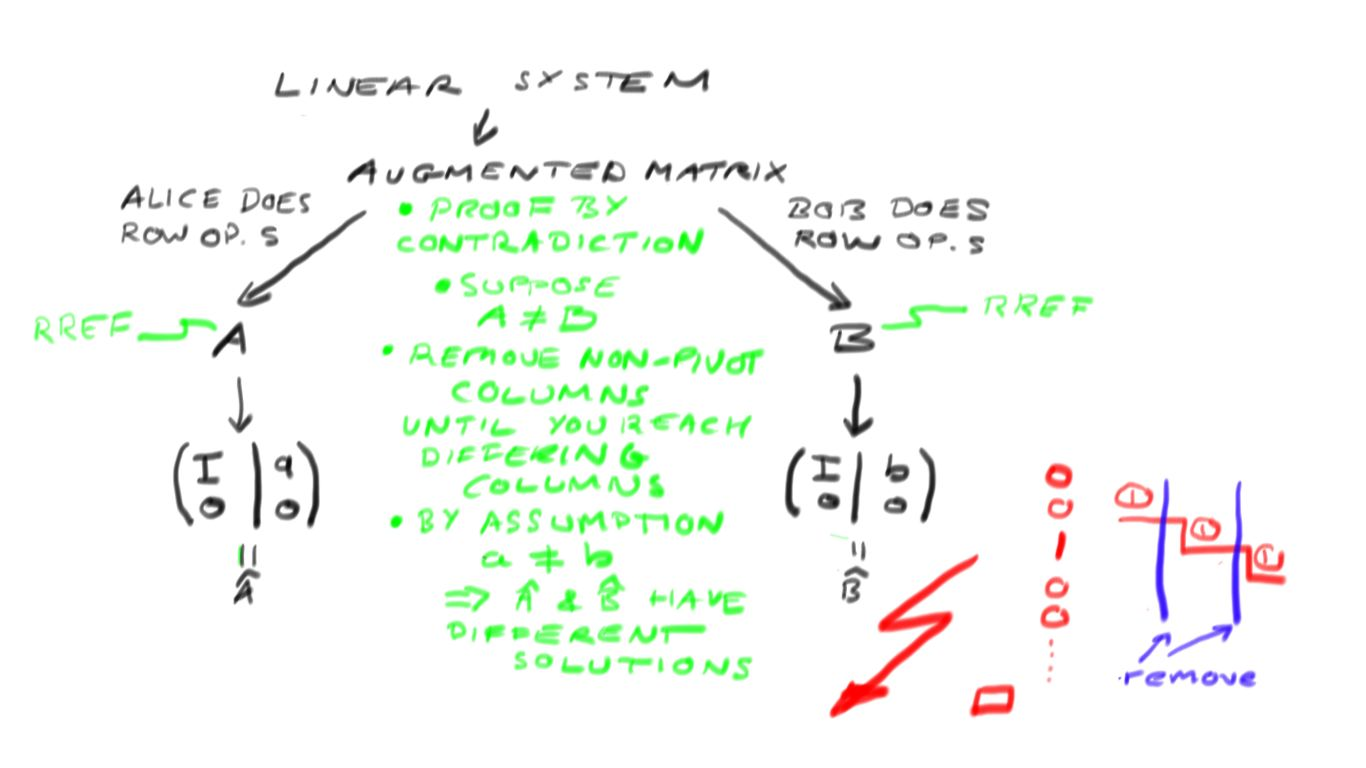
\includegraphics[scale=.3]{RREF_unique.jpg}
\end{center}

In words: we start with a linear system and convert it to an augmented matrix. Then, because we are studying a uniqueness
statement, we try a proof by contradiction. That is the  method where to show that a statement is true, you try to demonstrate that
the opposite of the statement leads to a contradiction. Here, the opposite statement to the theorem would be to find
two different RREFs for the same system.

Suppose, therefore, that Alice and Bob do find different RREF augmented matrices called $A$ and $B$. 
Then remove all the non-pivot columns  from $A$ and $B$  until you hit the first column that differs. Record that in the last column
and call the results $\widehat A$ and $\widehat B$. Removing columns
does change the solution sets, but it does not ruin row equivalence, so  $\widehat A$ and $\widehat B$ have the same solution sets.

Now, because we left only the pivot columns (plus the first column that differs) we have
$$\hat{A}=\begin{amatrix}{1}
I_N & a\\
0 & 0
\end{amatrix} \mbox{ and } \hat{B}=\begin{amatrix}{1}
I_N & b\\
0 & 0
\end{amatrix}\, ,$$ where $I_N$ is an identity matrix and $a$ and $b$ are column vectors.
Importantly, by assumption,
$$
a\neq b\, .
$$
So if we try to wrote down the solution sets for $\widehat A$ and $\widehat B$ they would be different.
But at all stages, we only performed operations that kept Alice's solution set the same as Bob's.
This is a contradiction so the proof is complete.
} % Closing brace for the font

\newpage



\subsection{\elemMatDetTitle: Hints for \hyperref[prob_inversion_number]{Problem~\ref*{prob_inversion_number}}}

%%%Insert this to get the typewriter font so it looks like a real movie script
{\ttfamily
\fontdimen2\font=0.4em
\fontdimen3\font=0.2em
\fontdimen4\font=0.1em
\fontdimen7\font=0.1em
\hyphenchar\font=`\-


\hypertarget{scripts_elementary_matrices_determinants_hint}{Here we will examine} the \hyperlink{inversion_number}{inversion number} and the effect of the transposition $\tau_{1,2}$ and $\tau_{2,4}$ on the permutation $\nu = [3, 4, 1, 2]$. Recall that the inversion number is basically the number of items out of order. So the inversion number of $\nu$ is $4$ since $3 > 1$ and $4 > 1$ and $3 > 2$ and $4 > 2$. Now we have $\tau_{1,2} \nu = [4, 3, 1, 2]$ by interchanging the first and second entries, and the inversion number is now $5$ since we now also have $4 > 3$. Next we have $\tau_{2,4} \nu = [3, 2, 1, 4]$ whose inversion number is $3$ since $3 > 2 > 1$. Finally we have $\tau_{1,2} \tau_{2,4} \nu = [2, 3, 1, 4]$ and the resulting inversion number is $2$ since $2 > 1$ and $3 > 1$. Notice how when we are applying $\tau_{i,j}$ the parity of the inversion number changes.


} % Closing bracket for font

\newpage



\subsection*{Planes}

%%%Insert this to get the typewriter font so it looks like a real movie script
{\ttfamily
\fontdimen2\font=0.4em
\fontdimen3\font=0.2em
\fontdimen4\font=0.1em
\fontdimen7\font=0.1em
\hyphenchar\font=`\-


%%%%put a hypertarget around the opening bit of text
\hypertarget{solution_sets_for_systems_of_linear_equations_planes}{Here we want} to describe the mathematics of planes in space.
The video is summarised by the following picture:
\begin{center}
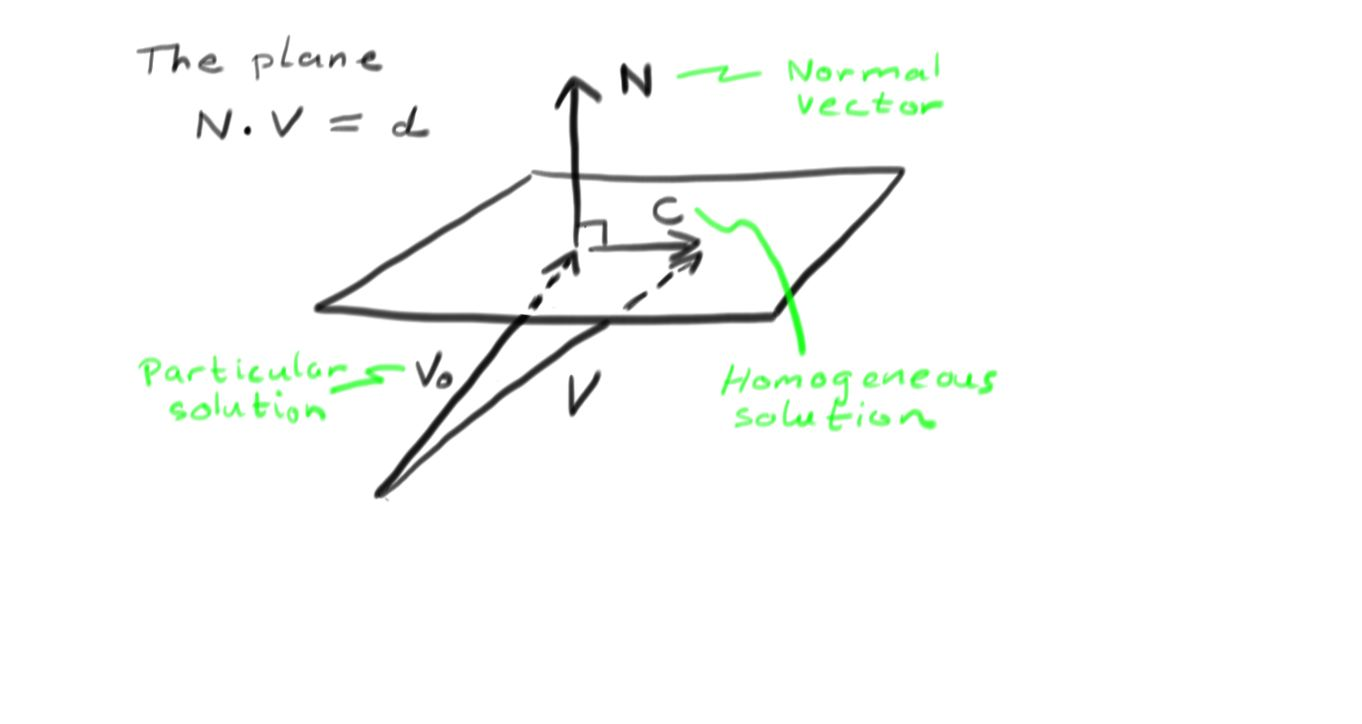
\includegraphics[scale=.2]{plane1eq.jpg}
\end{center}
A plane is often called ${\mathbb R}^2$ because it is spanned by  two coordinates, and space is called ${\mathbb R}^3$ and has three coordinates, 
usually called $(x,y,z)$. The equation for a plane is
$$
ax+by+cz=d\, .
$$
Lets simplify this by calling $V=(x,y,z)$ the vector of unknowns and $N=(a,b,c)$. Using the dot product in ${\mathbb R}^3$
we have
$$
N\dotprod V = d\, .
$$
Remember that when vectors are perpendicular their dot products vanish. {\it I.e.} $U\dotprod V = 0 \Leftrightarrow U \perp V$.
This means that if a vector $V_0$ solves our equation $N\dotprod V =d$, then so too does $V_0+C$ whenever $C$ is perpendicular to $N$.
This is because
$$N\dotprod (V_0+C) = N\dotprod V_0 + N\dotprod C = d + 0 = d\, .$$
But $C$ is ANY vector perpendicular to $N$, so all the possibilities for $C$ span a plane whose normal vector is $N$. Hence we have shown that 
solutions to the equation $ax+by+cz=0$ are a plane with normal vector $N=(a,b,c)$.



%%%%don't forget to close the bracket so the stuff after your file doesn't look like a movie!
}

%\newpage



\subsection*{Pictures and Explanation}

%%%Insert this to get the typewriter font so it looks like a real movie script
{\ttfamily
\fontdimen2\font=0.4em
\fontdimen3\font=0.2em
\fontdimen4\font=0.1em
\fontdimen7\font=0.1em
\hyphenchar\font=`\-


%%%%put a hypertarget around the opening bit of text
\hypertarget{solution_sets_for_systems_of_linear_equations_overview}{This video considers solutions sets}
for linear systems with three unknowns. These are often called $(x,y,z)$ and label points in ${\mathbb R}^3$.
Lets work case by case:

\begin{itemize}
\item If you have no equations at all, then any $(x,y,z)$ is a solution, so the solution set is  all of~${\mathbb R}^3$.
The picture looks a little silly:
\begin{center}
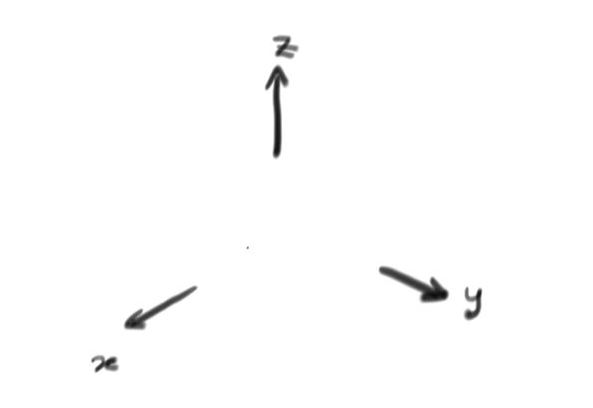
\includegraphics[alt={Three basis vectors x, y, and z.},scale=.15]{all_of_R3.jpg}
\end{center}
\item For a single equation, the solution is a plane. This is explained in this \href{\videourl solution_sets_for_systems_of_linear_equations_planes.mp4}{video}
or the accompanying \hyperlink{solution_sets_for_systems_of_linear_equations_planes}{script}. The picture looks like this:
\begin{center}
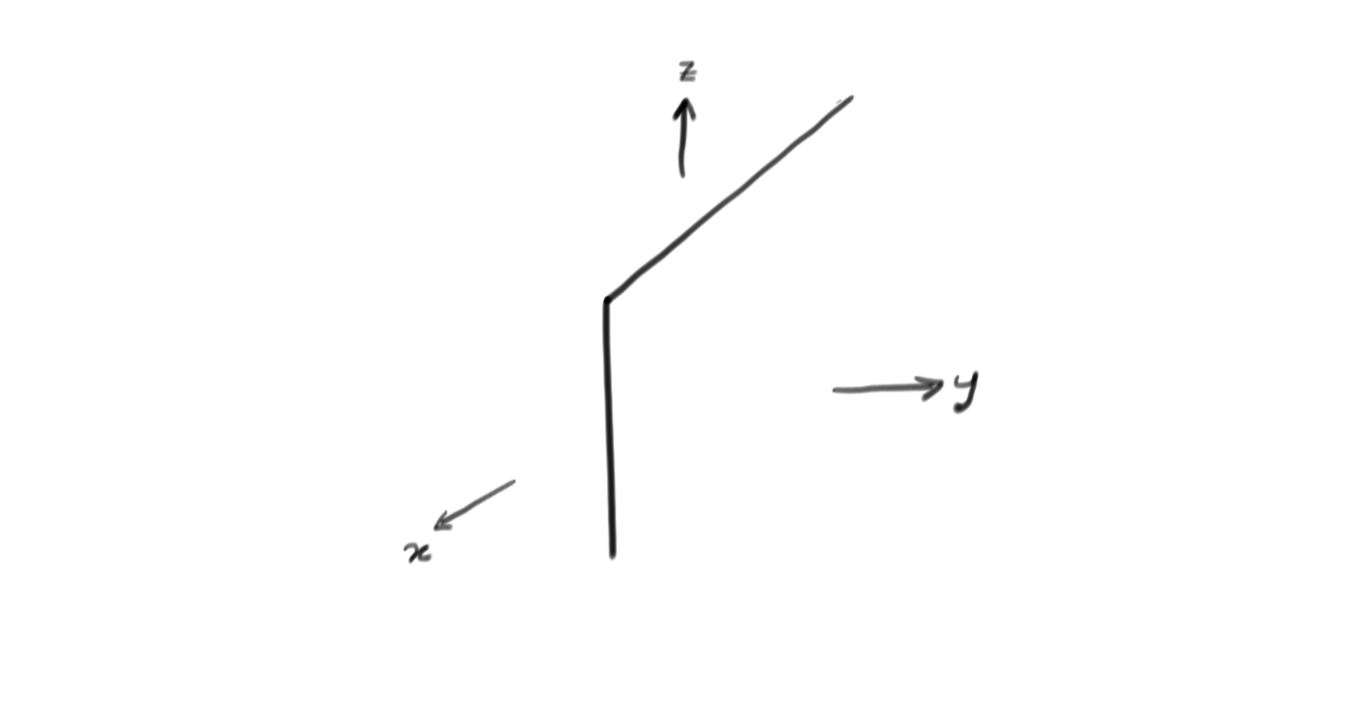
\includegraphics[alt={A plane in three dimensions, which is difficult to draw.},scale=.18]{plane_in_R3.jpg}
\end{center}
\item For two equations, we must look at two planes. These usually intersect along a line, so the solution set will also (usually) be a line:~\begin{center}
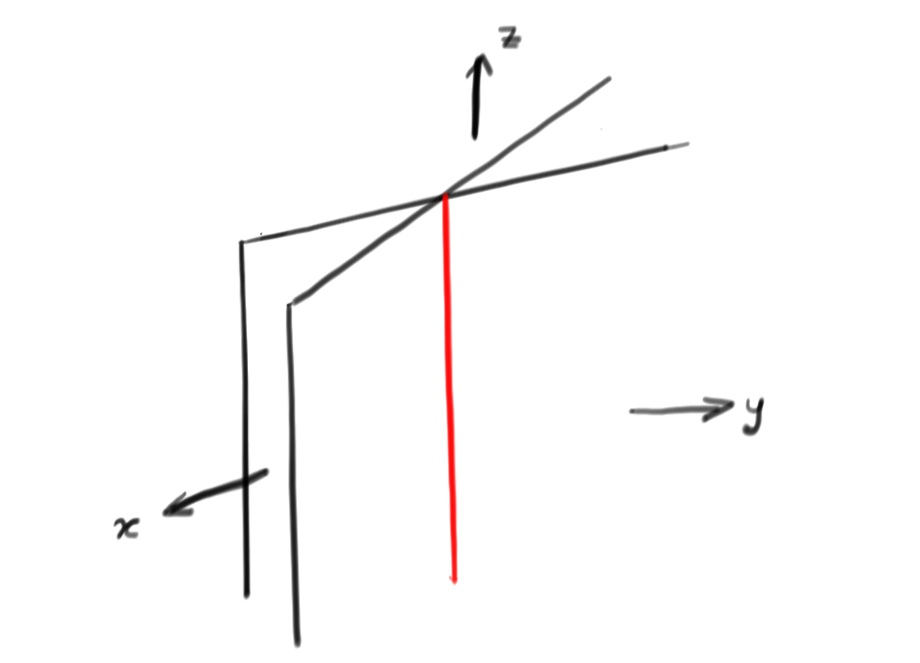
\includegraphics[alt={Two planes in space intersecting in a line.},scale=.18]{two_planes_in_R3.jpg}
\end{center}
\item For three equations, most often their intersection will be a single point so the solution will then be unique:
\begin{center}
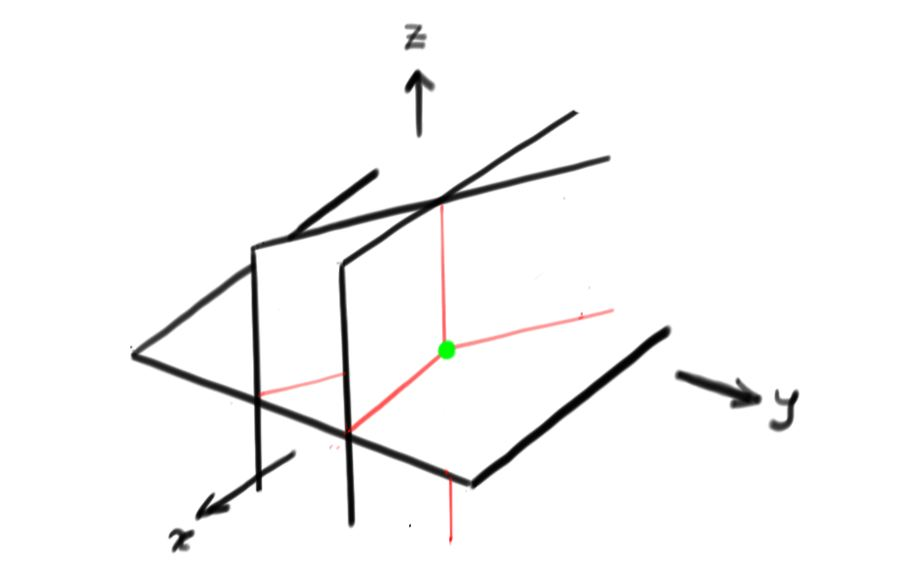
\includegraphics[alt={Three planes in space intersecting in a point.},scale=.17]{three_planes_in_R3.jpg}
\end{center}
\item Of course stuff can go wrong. Two different looking equations could determine the same plane, or worse equations could be inconsistent.
If the equations are inconsistent, there will be no solutions at all. For example, if you had four equations determining four parallel planes the solution set would be empty. This looks like this:
\begin{center}
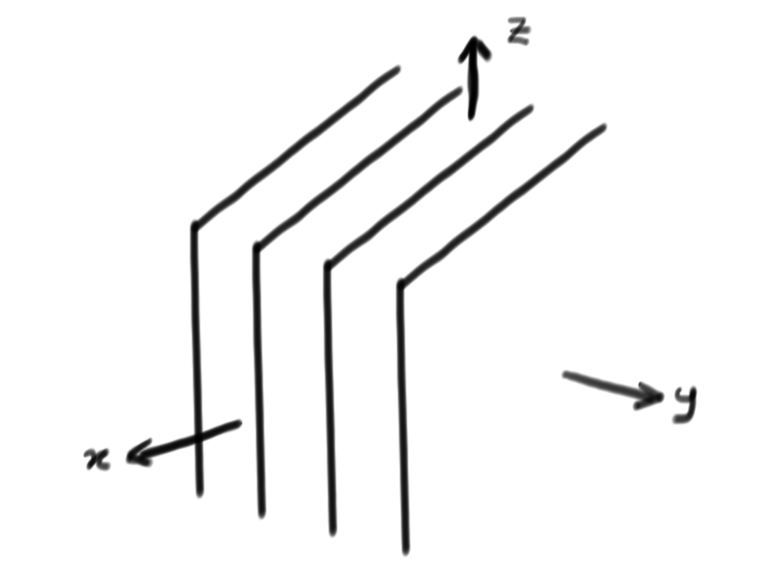
\includegraphics[alt={Four parallel planes in space.},scale=.16]{four_planes_in_R3.jpg}
\end{center}
\end{itemize}



%%%%don't forget to close the bracket so the stuff after your file doesn't look like a movie!
}

%\newpage



\subsection*{Matrix Exponential Example}

{\ttfamily
\fontdimen2\font=0.4em
\fontdimen3\font=0.2em
\fontdimen4\font=0.1em
\fontdimen7\font=0.1em
\hyphenchar\font=`\-

\hypertarget{properties_of_matrices_example}{This video} shows you
how to compute
\[
\exp\begin{pmatrix}0&\theta\\-\theta & 0\end{pmatrix}
\, .
\]
For this we need to remember that the matrix exponential is defined by its power series
\[
\exp M := I + M + \frac1{2!} M^2 + \frac1{3!} M^3+\cdots\, .
\]
Now lets call 
\[\begin{pmatrix}0&\theta\\-\theta & 0\end{pmatrix}=i\theta\]
where the {\it matrix} 
\[
i:=\begin{pmatrix}0&1\\-1 & 0\end{pmatrix}
\]
and by matrix multiplication is seen to obey
\[
i^2 =-I\, ,\qquad i^3=-i\, , i^4 = I\, .
\]
Using these facts we compute by organizing terms according to whether they have an $i$ or not:
\begin{eqnarray*}
\exp i\theta &=& I + \frac 1{2!}\, \theta^2 (-I) + \frac 1{4!} \,(+I) + \cdots \\
&+&i \theta + \frac1{3!} \,\theta^3 (-i) + \frac 1{5!} \,i+\cdots\\[2mm]
&=& I ( 1-\frac 1{2!}\, \theta^2  + \frac 1{4!}\,\theta^4  + \cdots)\\
&+&i( \theta- \frac1{3!}\, \theta^3  + \frac 1{5!}\,\theta^5 +\cdots)\\[2mm]
&=&I\cos\theta + i \sin\theta \\[2mm]
&=&\begin{pmatrix}\cos\theta & \sin\theta \\ -\sin\theta & \cos\theta\end{pmatrix}\, .
\end{eqnarray*}
Here we used the familiar Taylor series for the cosine and sine functions. A fun thing to think about is how the above matrix
acts on vector in the plane.


} % Closing brace for the font

%\newpage



\subsection{\elemMatDetTitle: Hints for \hyperref[prob_inversion_number]{Problem~\ref*{prob_inversion_number}}}

%%%Insert this to get the typewriter font so it looks like a real movie script
{\ttfamily
\fontdimen2\font=0.4em
\fontdimen3\font=0.2em
\fontdimen4\font=0.1em
\fontdimen7\font=0.1em
\hyphenchar\font=`\-


\hypertarget{scripts_elementary_matrices_determinants_hint}{Here we will examine} the \hyperlink{inversion_number}{inversion number} and the effect of the transposition $\tau_{1,2}$ and $\tau_{2,4}$ on the permutation $\nu = [3, 4, 1, 2]$. Recall that the inversion number is basically the number of items out of order. So the inversion number of $\nu$ is $4$ since $3 > 1$ and $4 > 1$ and $3 > 2$ and $4 > 2$. Now we have $\tau_{1,2} \nu = [4, 3, 1, 2]$ by interchanging the first and second entries, and the inversion number is now $5$ since we now also have $4 > 3$. Next we have $\tau_{2,4} \nu = [3, 2, 1, 4]$ whose inversion number is $3$ since $3 > 2 > 1$. Finally we have $\tau_{1,2} \tau_{2,4} \nu = [2, 3, 1, 4]$ and the resulting inversion number is $2$ since $2 > 1$ and $3 > 1$. Notice how when we are applying $\tau_{i,j}$ the parity of the inversion number changes.


} % Closing bracket for font

\newpage


\newpage

\section*{Webwork Links}

\reading{1}{1}

\reading{1}{1}

\reading{2}{1}

\reading{2}{2}

\reading{3}{1}

\reading{4}{1}

\reading{4}{2}


\begin{center}\href{http://webwork.math.ucdavis.edu/webwork2/MAT22A-Waldron-Winter-2012/Homework0-Background/}{Background homework set}\end{center}

\begin{center}\href{http://webwork.math.ucdavis.edu/webwork2/MAT22A-Waldron-Winter-2012/Homework1-LinearSystems-waldron}{Linear Systems}\end{center}

\begin{center}\href{http://webwork.math.ucdavis.edu/webwork2/MAT22A-Waldron-Winter-2012/Homework2-SolnSets-Vectors-waldron/}{Solution Sets}\end{center}

\end{document}
